\documentclass{article}

\usepackage[margin=1.2cm, top=1cm, bottom=1.8cm]{geometry}
\pagestyle{plain}
\linespread{1.25}

\usepackage{fontspec}
\usepackage{unicode-math}
\usepackage[main=greek, english]{babel}

\setmainfont{CMU Serif}
\setsansfont{CMU Sans Serif}
\setmonofont{CMU Typewriter Text}
\setmathfont{Latin Modern Math}

\usepackage{amsmath, enumitem}
\usepackage{dirtytalk, caption, subcaption, array, graphicx}
\usepackage{booktabs}
\usepackage{placeins}
\usepackage{titlesec}
\usepackage{soul}
\usepackage[unicode]{hyperref}
\usepackage{verbatim}

\usepackage{pdfpages}

\usepackage{tikz}
\usetikzlibrary{arrows.meta, positioning}

\graphicspath{{../benchmarks/diagrams/}{exercises/1st/benchmarks/diagrams/}{./}}

\hypersetup{
    hidelinks,
    bookmarksopen=true,
    bookmarksnumbered=true,
    pdftitle={Προηγμένα Θέματα Αρχιτεκτονικής Υπολογιστών - 1η Εργαστηριακή Άσκηση},
    pdfauthor={Πέππας Μιχαήλ-Αθανάσιος}
}

\newcolumntype{P}[1]{>{\centering\arraybackslash}p{#1}}
\titleformat*{\subsubsection}{\large\bfseries}

\begin{document}

\begin{center}
    {
    \Large
    {
    \textbf{ΕΘΝΙΚΟ ΜΕΤΣΟΒΙΟ ΠΟΛΥΤΕΧΝΕΙΟ\\
    ΣΧΟΛΗ ΗΛΕΚΤΡΟΛΟΓΩΝ ΜΗΧΑΝΙΚΩΝ\\
    ΚΑΙ ΜΗΧΑΝΙΚΩΝ ΥΠΟΛΟΓΙΣΤΩΝ}
    }

    \vspace{1.5cm}
    \rule{18cm}{0.5pt}

    Τομέας Τεχνολογίας, Πληροφορικής και Υπολογιστών\\
    Εργαστήριο Υπολογιστικών Συστημάτων\\

    \rule{18cm}{0.5pt}

    \textbf{Προηγμένα Θέματα Αρχιτεκτονικής Υπολογιστών}\\
    \textbf{$\mathbf{1^{η}}$ Εργαστηριακή Άσκηση}\\
    }
\end{center}

\vspace{0.8cm}
\begin{center}
\IfFileExists{EMP Logo.png}{\includegraphics[width=7cm]{EMP Logo.png}}{\vspace{2.5cm}}
\end{center}

\Large
{
\vspace{0.8cm}
\noindent
\textbf{Στοιχεία Φοιτητή}
\begin{itemize}
    \item Όνομα: Πέππας Μιχαήλ-Αθανάσιος
    \item Αριθμός Μητρώου: 03121026
    \item Email: el21026@mail.ntua.gr
    \item Ημερομηνία Παράδοσης Αναφοράς: 05.05.2026
\end{itemize}
}

\newpage
\tableofcontents

\newpage
\section{Μεθοδολογία, μετρικές και έλεγχος δεδομένων}

Στην παρούσα εργαστηριακή άσκηση μελετήθηκαν μηχανισμοί πρόβλεψης εντολών άλματος, με στόχο να αξιολογηθεί η επίδραση διαφορετικών μικροαρχιτεκτονικών επιλογών στην ακρίβεια πρόβλεψης. Η πρόβλεψη διακλαδώσεων είναι κρίσιμη για τους σύγχρονους επεξεργαστές, επειδή τα control hazards μπορούν να οδηγήσουν σε stalls και να μειώσουν σημαντικά τον ρυθμό προσκόμισης και εκτέλεσης εντολών. Ειδικά σε βαθιά pipelines, το κόστος μιας λανθασμένης πρόβλεψης αυξάνεται, αφού περισσότερες λανθασμένα προσκομισμένες ή εκτελεσμένες εντολές πρέπει να ακυρωθούν.

Για την εκτέλεση των πειραμάτων χρησιμοποιήθηκε το εργαλείο \foreignlanguage{english}{PIN}, δηλαδή ένα εργαλείο \foreignlanguage{english}{dynamic binary instrumentation}. Το \foreignlanguage{english}{PIN} επιτρέπει την εισαγωγή κώδικα παρακολούθησης κατά την εκτέλεση ενός προγράμματος, χωρίς να απαιτείται τροποποίηση του ίδιου του εκτελέσιμου. Στην άσκηση αξιοποιήθηκαν δύο βασικά \foreignlanguage{english}{pintools}: το \texttt{cslab\_branch\_stats.cpp}, το οποίο συλλέγει στατιστικά για τις εντολές άλματος, και το \texttt{cslab\_branch.cpp}, το οποίο προσομοιώνει διαφορετικούς μηχανισμούς πρόβλεψης, BTB και RAS. Στο δεύτερο εργαλείο προστέθηκαν οι απαιτούμενες διαμορφώσεις ώστε να καλύπτονται τα ερωτήματα 5.3--5.7.

Η εκφώνηση ορίζει ότι τα ερωτήματα 5.3--5.6 εκτελούνται με τα \texttt{train} inputs, ενώ στο 5.2 ζητείται ανάλυση τόσο για τα \texttt{train} όσο και για τα \texttt{ref} inputs. Το ερώτημα 5.7 λειτουργεί ως έλεγχος γενίκευσης: μετά την επιλογή των καλύτερων μηχανισμών από το 5.6.2, οι ίδιοι predictors εκτελούνται και στα \texttt{ref} inputs, ώστε να φανεί αν τα συμπεράσματα από τα μικρότερα \texttt{train} inputs παραμένουν αξιόπιστα σε μεγαλύτερες και πιο αντιπροσωπευτικές εκτελέσεις.

Η βασική μετρική αξιολόγησης για τους μηχανισμούς πρόβλεψης κατεύθυνσης είναι το \foreignlanguage{english}{direction MPKI}:
\[
    \text{direction MPKI} =
    \frac{\text{direction mispredictions}}{\text{total instructions}} \cdot 1000.
\]
Η μετρική αυτή μετρά πόσες λανθασμένες προβλέψεις κατεύθυνσης αντιστοιχούν σε κάθε χίλιες εκτελεσμένες εντολές. Έτσι, δεν εξετάζει μόνο το ποσοστό αποτυχίας ανά branch, αλλά κανονικοποιεί το αποτέλεσμα ως προς το συνολικό μέγεθος της εκτέλεσης.

Στην αναφορά χρησιμοποιήθηκαν δύο συμπληρωματικοί μέσοι όροι. Ο αριθμητικός μέσος του MPKI δίνει ίσο βάρος σε κάθε benchmark και χρησιμοποιείται ως κύριο κριτήριο επιλογής, επειδή αποτυπώνει πιο καθαρά τη συμπεριφορά ενός predictor στο σύνολο των μετροπρογραμμάτων, χωρίς να κυριαρχούν τα benchmarks με τις περισσότερες δυναμικές εντολές. Παράλληλα, χρησιμοποιείται και το \foreignlanguage{english}{aggregate MPKI}:
\[
    \text{aggregate MPKI} =
    \frac{\sum \text{mispredictions}}{\sum \text{instructions}} \cdot 1000.
\]
Το aggregate MPKI δίνει ίσο βάρος σε κάθε δυναμική εντολή και επομένως επηρεάζεται περισσότερο από τα benchmarks με μεγαλύτερο πλήθος εκτελεσμένων εντολών.

Δεν χρησιμοποιήθηκε γεωμετρικός μέσος για το MPKI. Ο γεωμετρικός μέσος είναι συνηθισμένος σε λόγους επίδοσης, όπως speedups, αλλά το MPKI είναι φυσική μετρική πλήθους αστοχιών ανά χίλιες εντολές. Επομένως, ο αριθμητικός μέσος και ο instruction-weighted μέσος έχουν σαφέστερη ερμηνεία στο συγκεκριμένο πλαίσιο. Με άλλα λόγια, εδώ δεν συγκρίνουμε λόγους επιτάχυνσης, αλλά κανονικοποιημένα πλήθη σφαλμάτων.

Πριν από τη συγγραφή των συμπερασμάτων έγινε έλεγχος πληρότητας των παραγόμενων αρχείων. Δεν εντοπίστηκαν missing ή unparseable raw outputs. Συνολικά υπήρχαν 22 outputs για το 5.2, 11 outputs για καθεμία από τις ενότητες 5.3, 5.4, 5.5, 5.6.1 και 5.6.2, καθώς και 11 \texttt{ref} outputs για το 5.7. Τα μόνα μη κενά stderr logs εμφανίστηκαν στο \texttt{416.gamess} και αντιστοιχούν σε γνωστές αριθμητικές προειδοποιήσεις ή τερματισμό του ίδιου του benchmark. Δεν επηρέασαν την εγκυρότητα των αποτελεσμάτων, αφού τα αντίστοιχα raw outputs έγιναν parse κανονικά.

\section{5.2 Ανάλυση εντολών άλματος}

\subsection{Σκοπός και μεθοδολογία}

Το πρώτο πειραματικό βήμα έχει κυρίως διαγνωστικό χαρακτήρα. Δεν αξιολογεί ακόμη κάποιον συγκεκριμένο predictor, αλλά καταγράφει το δυναμικό μίγμα των εντολών άλματος για κάθε benchmark. Αυτό είναι απαραίτητο, επειδή η επίδοση ενός μηχανισμού πρόβλεψης δεν εξαρτάται μόνο από την ακρίβειά του, αλλά και από το πόσο συχνά εμφανίζονται branches και από το είδος αυτών των branches.

Για κάθε benchmark μετρήθηκαν οι συνολικές εντολές, οι συνολικές εντολές άλματος και η κατανομή των branches στις κατηγορίες \foreignlanguage{english}{conditional taken}, \foreignlanguage{english}{conditional not-taken}, \foreignlanguage{english}{unconditional}, \foreignlanguage{english}{calls} και \foreignlanguage{english}{returns}. Η συχνότητα εμφάνισης branches υπολογίστηκε ως:
\[
    \text{branch frequency} =
    \frac{\text{total branches}}{\text{total instructions}} \cdot 100\%.
\]

\begin{figure}[htbp]
    \centering
    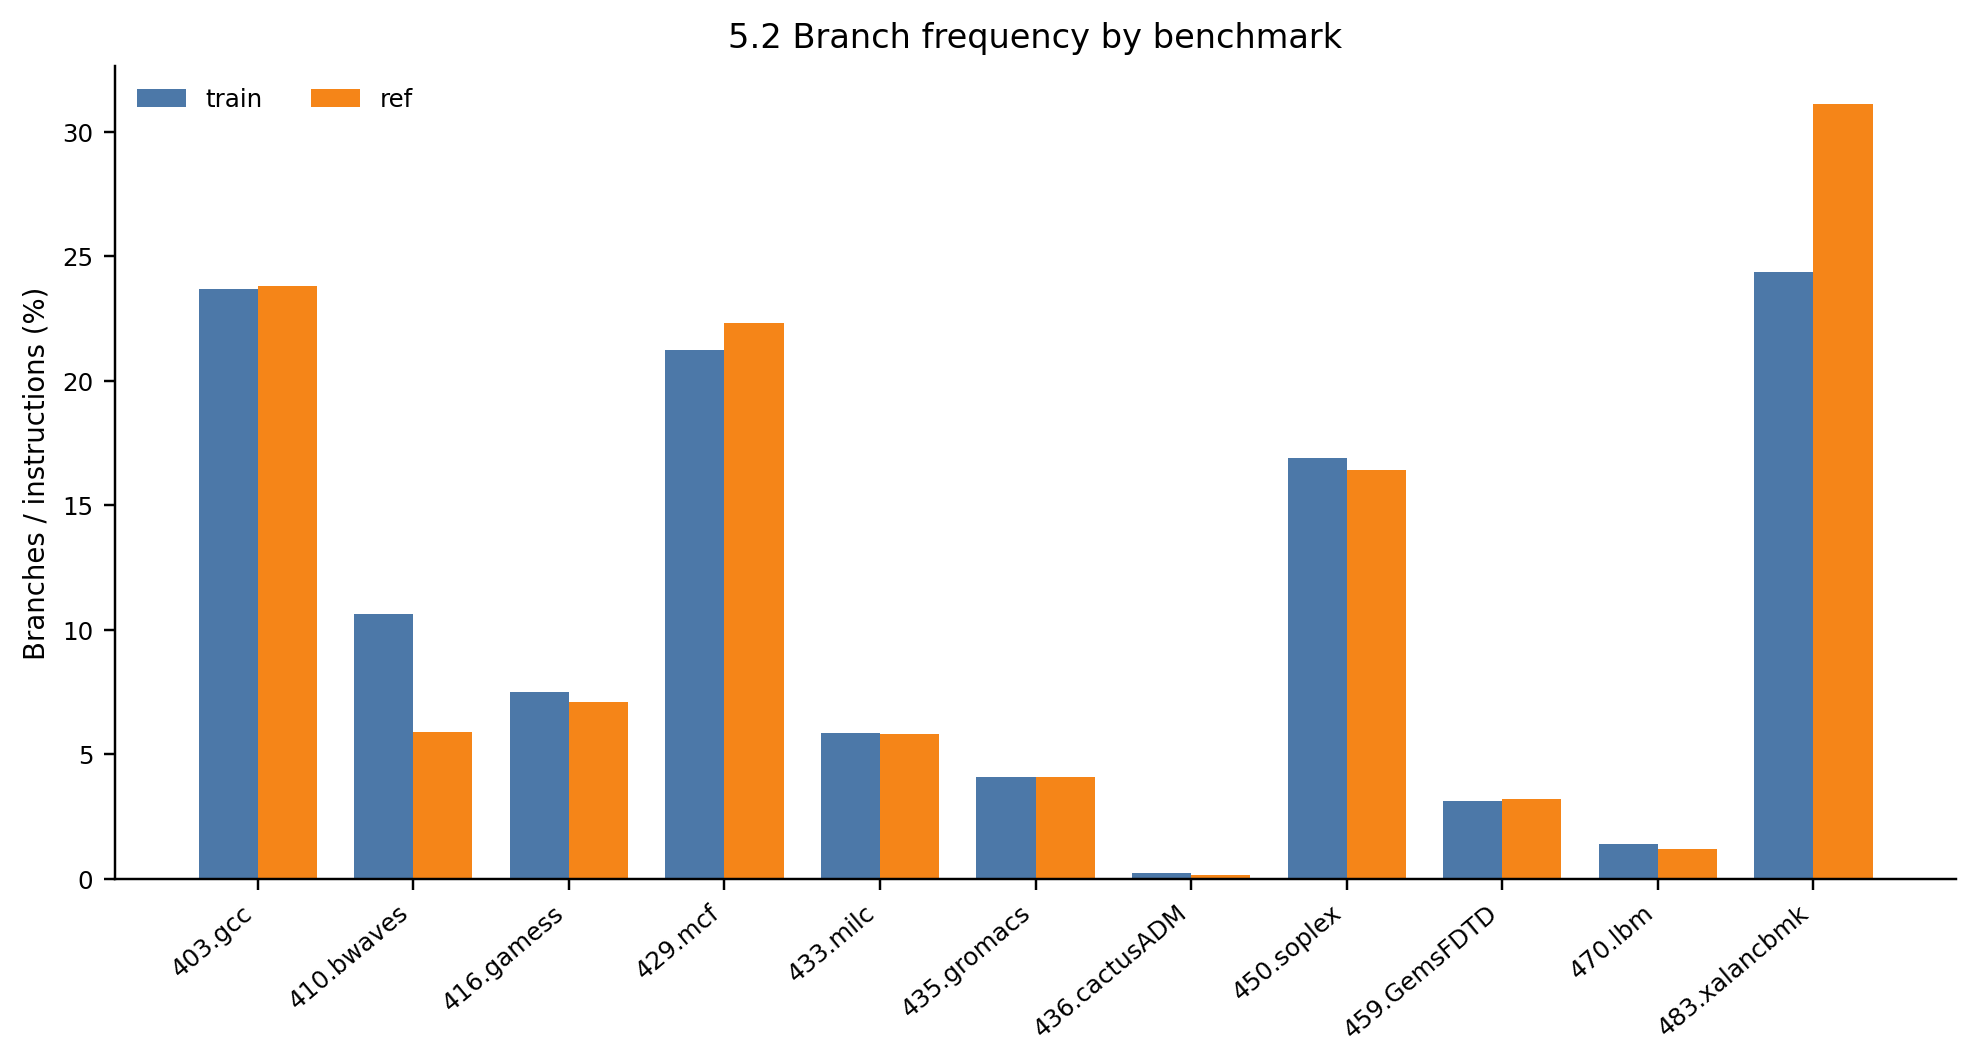
\includegraphics[width=0.95\linewidth]{5_2_branch_frequency.png}
    \caption{Συχνότητα εντολών άλματος για \texttt{train} και \texttt{ref} inputs.}
    \label{fig:branch_frequency}
\end{figure}

Από το Σχήμα~\ref{fig:branch_frequency} φαίνεται ότι τα benchmarks δεν έχουν την ίδια πυκνότητα εντολών άλματος. Στο \texttt{train} input, τα benchmarks με τη μεγαλύτερη συχνότητα branches είναι τα \texttt{483.xalancbmk} με 24.37\%, \texttt{403.gcc} με 23.69\%, \texttt{429.mcf} με 21.22\% και \texttt{450.soplex} με 16.89\%. Αντίθετα, τα \texttt{436.cactusADM} και \texttt{470.lbm} έχουν πολύ μικρό branch frequency, 0.21\% και 1.41\% αντίστοιχα.

Η ίδια γενική εικόνα παραμένει και στα \texttt{ref} inputs, αν και υπάρχουν ορισμένες σημαντικές διαφοροποιήσεις. Η πιο χαρακτηριστική περίπτωση είναι το \texttt{483.xalancbmk}, του οποίου το branch frequency αυξάνεται στο 31.10\%. Αυτό σημαίνει ότι, για το συγκεκριμένο input, το benchmark επιβαρύνει ακόμη περισσότερο τον μηχανισμό πρόβλεψης διακλαδώσεων.

Η παρατήρηση αυτή είναι σημαντική για την ερμηνεία του MPKI. Δύο benchmarks μπορεί να έχουν παρόμοιο ποσοστό αστοχίας ανά branch, αλλά διαφορετικό MPKI, αν το ένα εκτελεί πολύ περισσότερα branches ανά χίλιες εντολές. Επομένως, το branch frequency συνδέει την καθαρή ακρίβεια πρόβλεψης με την πραγματική επίδραση στο instruction stream.

\begin{figure}[htbp]
    \centering
    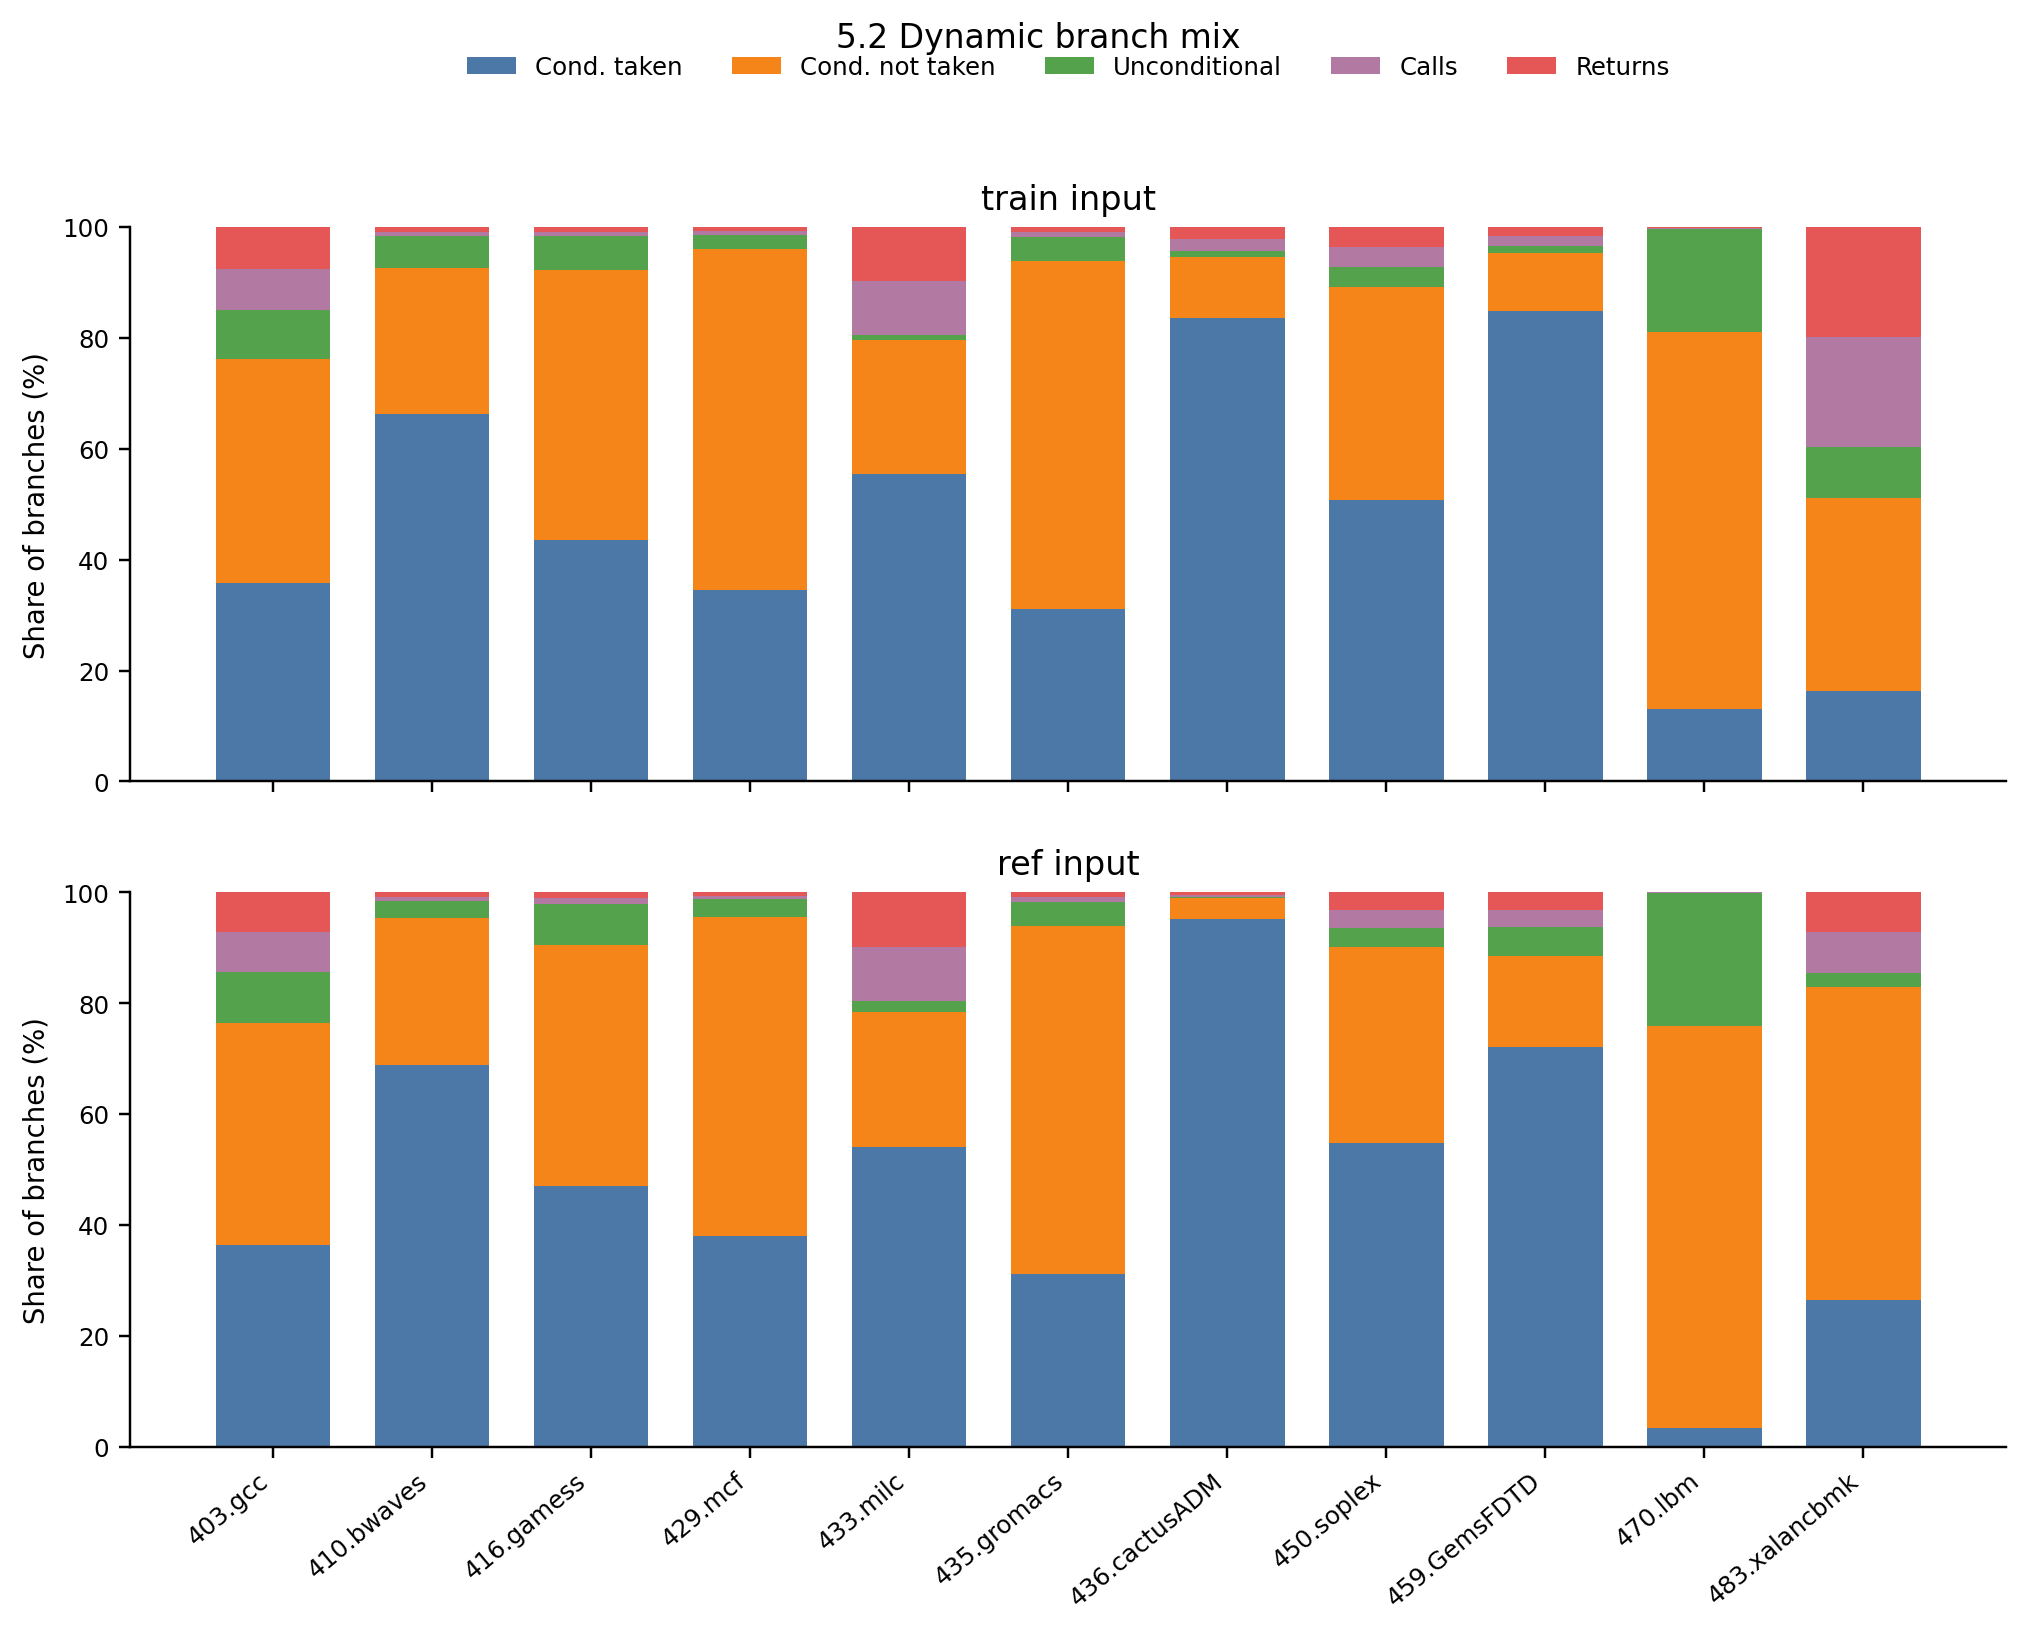
\includegraphics[width=0.95\linewidth]{5_2_branch_mix.png}
    \caption{Μίγμα κατηγοριών branches ως ποσοστό των συνολικών branches.}
    \label{fig:branch_mix}
\end{figure}

Το Σχήμα~\ref{fig:branch_mix} παρουσιάζει το μίγμα των διαφορετικών κατηγοριών branches. Στα περισσότερα benchmarks κυριαρχούν τα conditional branches, όπως αναμένεται, αφού αυτά είναι τα branches για τα οποία απαιτείται πρόβλεψη κατεύθυνσης. Ωστόσο, η κατανομή δεν είναι ίδια σε όλα τα benchmarks.

Για παράδειγμα, στο \texttt{483.xalancbmk} το \texttt{train} input έχει μεγάλο ποσοστό calls και returns, περίπου 19.82\% το καθένα. Άρα, για το συγκεκριμένο benchmark αναμένεται να έχει μεγάλη σημασία και ο μηχανισμός RAS, αφού οι επιστροφές από συναρτήσεις αποτελούν σημαντικό μέρος των δυναμικών branches. Αντίθετα, το \texttt{470.lbm} έχει χαμηλό branch frequency, αλλά σχετικά μεγάλο ποσοστό unconditional branches, 18.61\% στο \texttt{train} και 24.05\% στο \texttt{ref}.

Συνεπώς, από το 5.2 προκύπτει ότι η αξιολόγηση δεν μπορεί να περιοριστεί μόνο σε έναν μηχανισμό. Χρειάζεται να εξεταστούν ξεχωριστά η πρόβλεψη κατεύθυνσης, η πρόβλεψη στόχου μέσω BTB και η πρόβλεψη επιστροφών μέσω RAS.

\FloatBarrier
\section{5.3 Μηχανισμοί n-bit πρόβλεψης και εναλλακτικά FSMs}

\subsection{Θεωρητικό υπόβαθρο}

Οι απλοί δυναμικοί μηχανισμοί πρόβλεψης χρησιμοποιούν ένα \foreignlanguage{english}{Branch History Table} (BHT). Το BHT είναι ένας πίνακας που προσπελαύνεται συνήθως με βάση χαμηλότερα bits του PC της εντολής branch. Κάθε εγγραφή περιέχει πληροφορία για την πρόσφατη συμπεριφορά του αντίστοιχου branch ή, πιο σωστά, των branches που χαρτογραφούνται στην ίδια εγγραφή.

Στους n-bit predictors, κάθε εγγραφή του BHT είναι ένας saturating up-down counter. Όταν το branch είναι taken, ο counter αυξάνεται μέχρι τη μέγιστη τιμή του, ενώ όταν είναι not-taken μειώνεται μέχρι το μηδέν. Η πρόβλεψη προκύπτει από το πιο σημαντικό bit του counter. Αν το πιο σημαντικό bit αντιστοιχεί στην άνω μισή περιοχή τιμών, η πρόβλεψη είναι taken, διαφορετικά είναι not-taken.

Το βασικό πλεονέκτημα του 2-bit predictor έναντι του 1-bit predictor είναι το υστέρηση. Σε ένα τυπικό loop branch, η δυναμική ακολουθία είναι:
\[
    T, T, T, \ldots, T, N.
\]
Ο 1-bit predictor αλλάζει πρόβλεψη αμέσως μετά το τελικό not-taken και, στην επόμενη είσοδο στο loop, κάνει ξανά λάθος. Αντίθετα, ένας 2-bit saturating counter χρειάζεται δύο διαδοχικές αντίθετες εκβάσεις για να αλλάξει από ισχυρή taken σε not-taken πρόβλεψη. Έτσι, αποφεύγει ένα μέρος των λαθών που προκαλούνται από την έξοδο των loops.

Το βασικό trade-off είναι ανάμεσα στο πλήθος των entries και στο πλήθος των bits ανά entry. Περισσότερα entries μειώνουν το aliasing, δηλαδή τη σύγκρουση διαφορετικών branches στην ίδια θέση του πίνακα. Περισσότερα bits ανά entry προσφέρουν μεγαλύτερη υστέρηση, αλλά απαιτούν περισσότερο χώρο και μπορεί να κάνουν τον predictor πιο αργό στην προσαρμογή όταν αλλάζει πραγματικά η συμπεριφορά ενός branch.

\subsection{5.3(i): Σταθερά 16K BHT entries}

Στο πρώτο υποερώτημα κρατήθηκε σταθερό το πλήθος των BHT entries στις 16K και μεταβλήθηκε μόνο το πλήθος bits ανά entry. Με αυτόν τον τρόπο εξετάζεται καθαρά η επίδραση της υστέρησης, χωρίς να αλλάζει το πλήθος των διαθέσιμων εγγραφών.

\begin{center}
\begin{tabular}{lrrr}
\toprule
Predictor & Bits & Mean MPKI & Aggregate MPKI \\
\midrule
\texttt{Nbit-16K-1} & 16384 & 12.229 & 10.516 \\
\texttt{Nbit-16K-2} & 32768 & 7.761 & 6.505 \\
\texttt{Nbit-16K-3} & 49152 & 7.622 & 6.459 \\
\texttt{Nbit-16K-4} & 65536 & 7.717 & 6.531 \\
\bottomrule
\end{tabular}
\captionof{table}{Αποτελέσματα μηχανισμών n-bit πρόβλεψης με 16K BHT entries.}
\label{tab:nbit_16k}
\end{center}

Από τον Πίνακα~\ref{tab:nbit_16k} φαίνεται ότι η μετάβαση από 1-bit σε 2-bit predictor προσφέρει πολύ μεγάλη βελτίωση. Ο αριθμητικός μέσος του MPKI μειώνεται από 12.229 σε 7.761, γεγονός που επιβεβαιώνει τη σημασία της υστέρησης. Ο 1-bit predictor αντιδρά πολύ γρήγορα σε κάθε αλλαγή έκβασης και για αυτό επηρεάζεται έντονα από μοτίβα όπως η έξοδος από loops.

Με σταθερά 16K entries και χωρίς περιορισμό συνολικού hardware, ο καλύτερος predictor είναι ο \texttt{Nbit-16K-3}, με mean MPKI 7.622. Η βελτίωση σε σχέση με τον \texttt{Nbit-16K-2} είναι όμως μικρή, περίπου 0.139 MPKI, ενώ το κόστος αυξάνεται κατά 50\%. Ο \texttt{Nbit-16K-4} δεν βελτιώνει περαιτέρω την επίδοση και μάλιστα έχει ελαφρώς χειρότερο mean MPKI από τον 3-bit predictor. Αυτό δείχνει ότι η πρόσθετη υστέρηση δεν είναι πάντα ωφέλιμη: όταν ο predictor γίνεται υπερβολικά αδρανής, καθυστερεί να προσαρμοστεί σε πραγματικές αλλαγές της συμπεριφοράς.

Επομένως, αν το ερώτημα διαβαστεί αυστηρά ως σύγκριση με σταθερό πλήθος entries, ο \texttt{Nbit-16K-3} είναι ο καλύτερος αριθμητικά. Από αρχιτεκτονική άποψη, όμως, ο \texttt{Nbit-16K-2} παραμένει πολύ ελκυστικός, επειδή βρίσκεται πολύ κοντά στην καλύτερη επίδοση με αισθητά μικρότερο κόστος.

\subsection{5.3(ii): Εναλλακτικά 2-bit FSMs του Nair}

Στο δεύτερο υποερώτημα εξετάστηκαν εναλλακτικές 4-state μηχανές πεπερασμένων καταστάσεων για 2-bit predictors. Η βασική ιδέα είναι ότι ένας 2-bit predictor δεν είναι υποχρεωτικά μόνο ο κλασικός saturating counter. Με τέσσερις καταστάσεις μπορούν να οριστούν πολλές διαφορετικές μεταβάσεις και διαφορετικές αντιστοιχίσεις καταστάσεων σε taken ή not-taken πρόβλεψη.

Η κωδικοποίηση ενός FSM, όπως \texttt{BCBAADCD:3}, περιγράφει τις μεταβάσεις των καταστάσεων \(A,B,C,D\) για τις δύο δυνατές εκβάσεις του branch. Ο αριθμός μετά την άνω-κάτω τελεία δηλώνει ποιες καταστάσεις προβλέπουν taken. Ο κλασικός saturating counter αντιστοιχεί στο \texttt{ABACBDCD:3} και στη δική μας υλοποίηση εκπροσωπείται από τον \texttt{Nbit-16K-2}.

\begin{figure}[htbp]
    \centering
    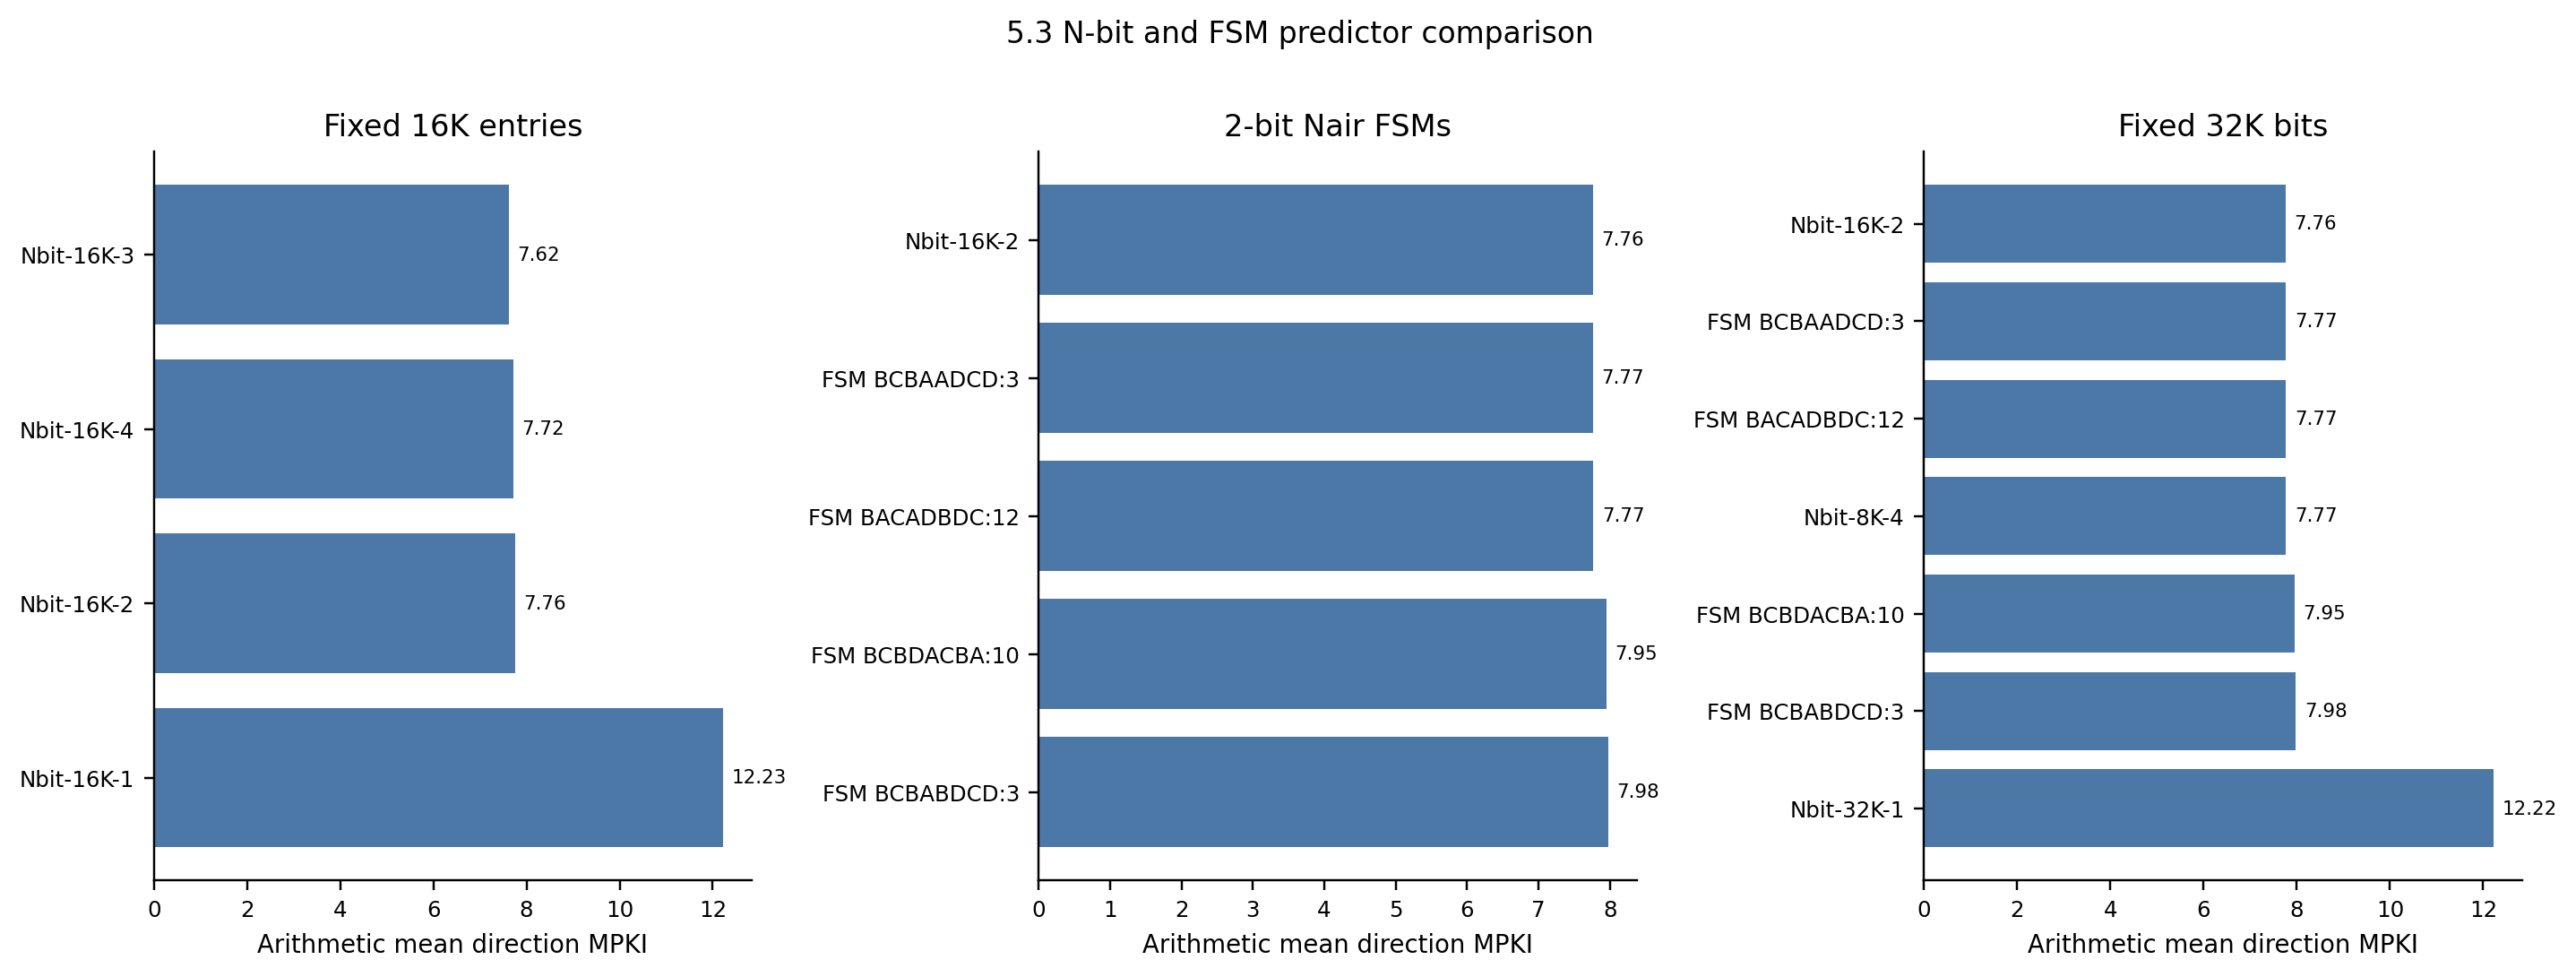
\includegraphics[width=0.98\linewidth]{5_3_predictor_groups.png}
    \caption{Σύγκριση μηχανισμών n-bit πρόβλεψης και Nair FSMs με αριθμητικό μέσο του direction MPKI.}
    \label{fig:nbit_groups}
\end{figure}

Τα αποτελέσματα του Σχήματος~\ref{fig:nbit_groups} δείχνουν ότι τα καλύτερα FSMs είναι πρακτικά ισοδύναμα με τον κλασικό 2-bit predictor. Συγκεκριμένα, ο \texttt{Nbit-16K-2} έχει mean MPKI 7.761, ο \texttt{FSM-16K-BCBAADCD-3} έχει 7.767 και ο \texttt{FSM-16K-BACADBDC-12} έχει 7.770. Οι διαφορές αυτές είναι πολύ μικρές για να θεωρηθεί ότι κάποιο πιο ειδικό FSM προσφέρει ουσιαστικό πλεονέκτημα.

Η ερμηνεία είναι ότι ο κλασικός saturating counter είναι ήδη πολύ κοντά στο βέλτιστο για τα συγκεκριμένα traces. Τα εναλλακτικά FSMs τροποποιούν τον τρόπο με τον οποίο ενσωματώνεται η υστέρηση, αλλά δεν αλλάζουν ριζικά τη διαθέσιμη πληροφορία. Επομένως, για το 5.3(ii) επιλέγεται ο \texttt{Nbit-16K-2}, όχι επειδή υπερέχει με μεγάλη διαφορά, αλλά επειδή συνδυάζει απλότητα, καθιερωμένη ερμηνεία και επίδοση ουσιαστικά ίδια με τα καλύτερα Nair FSMs.

\subsection{5.3(iii): Σταθερό hardware budget 32K bits}

Στο τρίτο υποερώτημα το hardware budget κρατήθηκε σταθερό στα 32K bits. Επομένως, η αύξηση των bits ανά counter μειώνει αναγκαστικά το πλήθος των entries:
\[
    1\text{-bit}: 32K \text{ entries}, \qquad
    2\text{-bit}: 16K \text{ entries}, \qquad
    4\text{-bit}: 8K \text{ entries}.
\]
Το πείραμα αυτό είναι πιο αντιπροσωπευτικό αρχιτεκτονικά, επειδή στην πράξη ο διαθέσιμος χώρος πάνω στο chip είναι περιορισμένος. Άρα, δεν αρκεί να αυξηθεί η υστέρηση, αλλά πρέπει να εξεταστεί και το κόστος αυτής της επιλογής σε aliasing.

\begin{figure}[htbp]
    \centering
    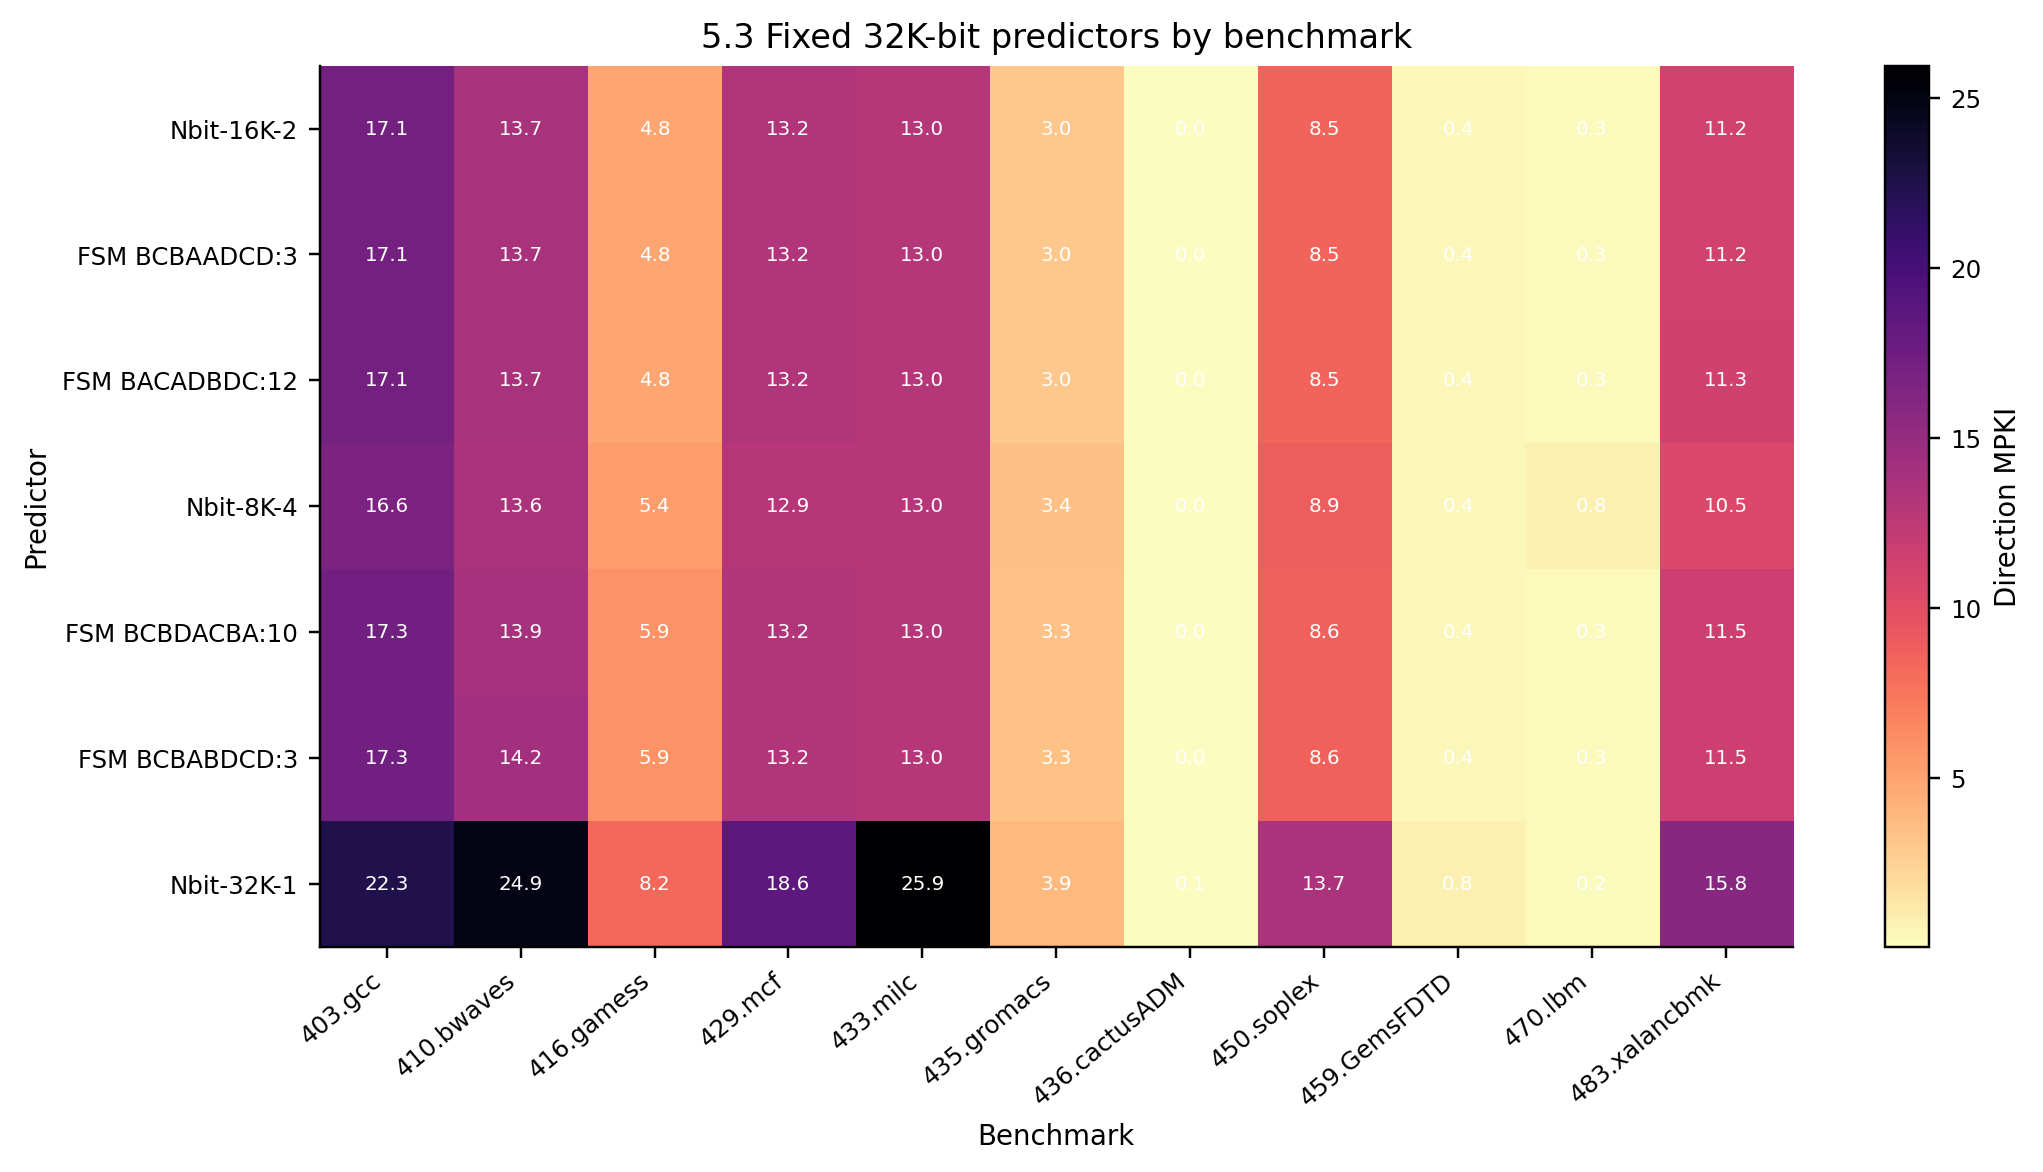
\includegraphics[width=0.98\linewidth]{5_3_fixed32_by_benchmark.png}
    \caption{Τιμή direction MPKI ανά benchmark για τους 7 μηχανισμούς του πειράματος fixed-32K.}
    \label{fig:nbit_fixed32_by_benchmark}
\end{figure}

\begin{center}
\begin{tabular}{lrr}
\toprule
Predictor & Mean MPKI & Aggregate MPKI \\
\midrule
\texttt{Nbit-16K-2} & 7.761 & 6.505 \\
\texttt{FSM-16K-BCBAADCD-3} & 7.767 & 6.506 \\
\texttt{FSM-16K-BACADBDC-12} & 7.770 & 6.520 \\
\texttt{Nbit-8K-4} & 7.770 & 6.569 \\
\texttt{FSM-16K-BCBDACBA-10} & 7.954 & 6.807 \\
\texttt{FSM-16K-BCBABDCD-3} & 7.979 & 6.858 \\
\texttt{Nbit-32K-1} & 12.217 & 10.516 \\
\bottomrule
\end{tabular}
\captionof{table}{Σύγκριση μηχανισμών πρόβλεψης με σταθερό κόστος 32K bits.}
\label{tab:fixed32}
\end{center}

Ο \texttt{Nbit-32K-1} έχει το μεγαλύτερο πλήθος entries, αλλά υστερεί σημαντικά, επειδή δεν διαθέτει υστέρηση. Αντίθετα, ο \texttt{Nbit-8K-4} έχει μεγαλύτερη υστέρηση, αλλά λιγότερα entries, άρα αυξημένο aliasing. Ο καλύτερος συμβιβασμός εμφανίζεται στον \texttt{Nbit-16K-2}, ο οποίος έχει το μικρότερο mean MPKI, 7.761, και πολύ καλή aggregate επίδοση, 6.505.

Το αποτέλεσμα αυτό είναι συνεπές με τη θεωρία. Τα 2 bits ανά entry είναι αρκετά για να αποφεύγονται οι συνηθισμένες διπλές αστοχίες των loops, ενώ το πλήθος των 16K entries παραμένει αρκετά μεγάλο ώστε να μη διογκώνεται υπερβολικά το aliasing. Για αυτόν τον λόγο ο \texttt{Nbit-16K-2} χρησιμοποιείται στη συνέχεια ως ο εκπρόσωπος των απλών n-bit predictors στο ερώτημα 5.6.2.

\FloatBarrier
\section{5.4 Μελέτη του BTB}

\subsection{Θεωρία, υλοποίηση και μετρικές}

Ο \foreignlanguage{english}{Branch Target Buffer} (BTB) χρησιμοποιείται για την πρόβλεψη του target PC των taken branches. Σε μια εντολή άλματος δεν αρκεί να προβλεφθεί αν το άλμα θα εκτελεστεί ή όχι. Αν προβλεφθεί taken, ο επεξεργαστής πρέπει να γνωρίζει άμεσα και τη διεύθυνση από την οποία θα συνεχίσει η προσκόμιση εντολών. Διαφορετικά, ακόμη και μια σωστή πρόβλεψη κατεύθυνσης δεν αρκεί για να αποφευχθεί καθυστέρηση στο frontend.

Στην υλοποίηση της άσκησης, ο BTB οργανώθηκε ως cache-like δομή. Κάθε εγγραφή περιέχει valid bit, tag, αποθηκευμένο target και πληροφορία αντικατάστασης LRU ανά set. Για κάθε οργάνωση ισχύει:
\[
    \text{sets} =
    \frac{\text{total entries}}{\text{associativity}}.
\]
Σε BTB hit, ο predictor προβλέπει taken και δίνει το αποθηκευμένο target. Σε BTB miss, η πρόβλεψη είναι not-taken. Οι εγγραφές ενημερώνονται μόνο όταν το πραγματικό αποτέλεσμα είναι taken, επειδή μόνο τότε υπάρχει ουσιαστικό target που πρέπει να αποθηκευτεί.

Η συμπεριφορά του BTB μοιάζει με τη συμπεριφορά μιας cache. Περισσότερα entries μειώνουν τα capacity misses, ενώ το μεγαλύτερο associativity μειώνει τα conflict misses. Ωστόσο, για σταθερό μέγεθος, η αύξηση του associativity μειώνει το πλήθος των sets και αυξάνει το κόστος των συγκρίσεων tags. Επομένως, υπάρχει trade-off ανάμεσα σε capacity, conflict behavior και πολυπλοκότητα.

Στο BTB διακρίνονται δύο είδη αστοχίας. Direction miss εμφανίζεται όταν η πρόβλεψη taken/not-taken είναι λανθασμένη. Target miss εμφανίζεται όταν η πρόβλεψη taken είναι σωστή, αλλά το αποθηκευμένο target είναι διαφορετικό από το πραγματικό target. Τα target misses είναι συνήθως πιο ειδική περίπτωση και σχετίζονται κυρίως με indirect branches ή branches των οποίων ο στόχος μεταβάλλεται δυναμικά.

\begin{figure}[htbp]
    \centering
    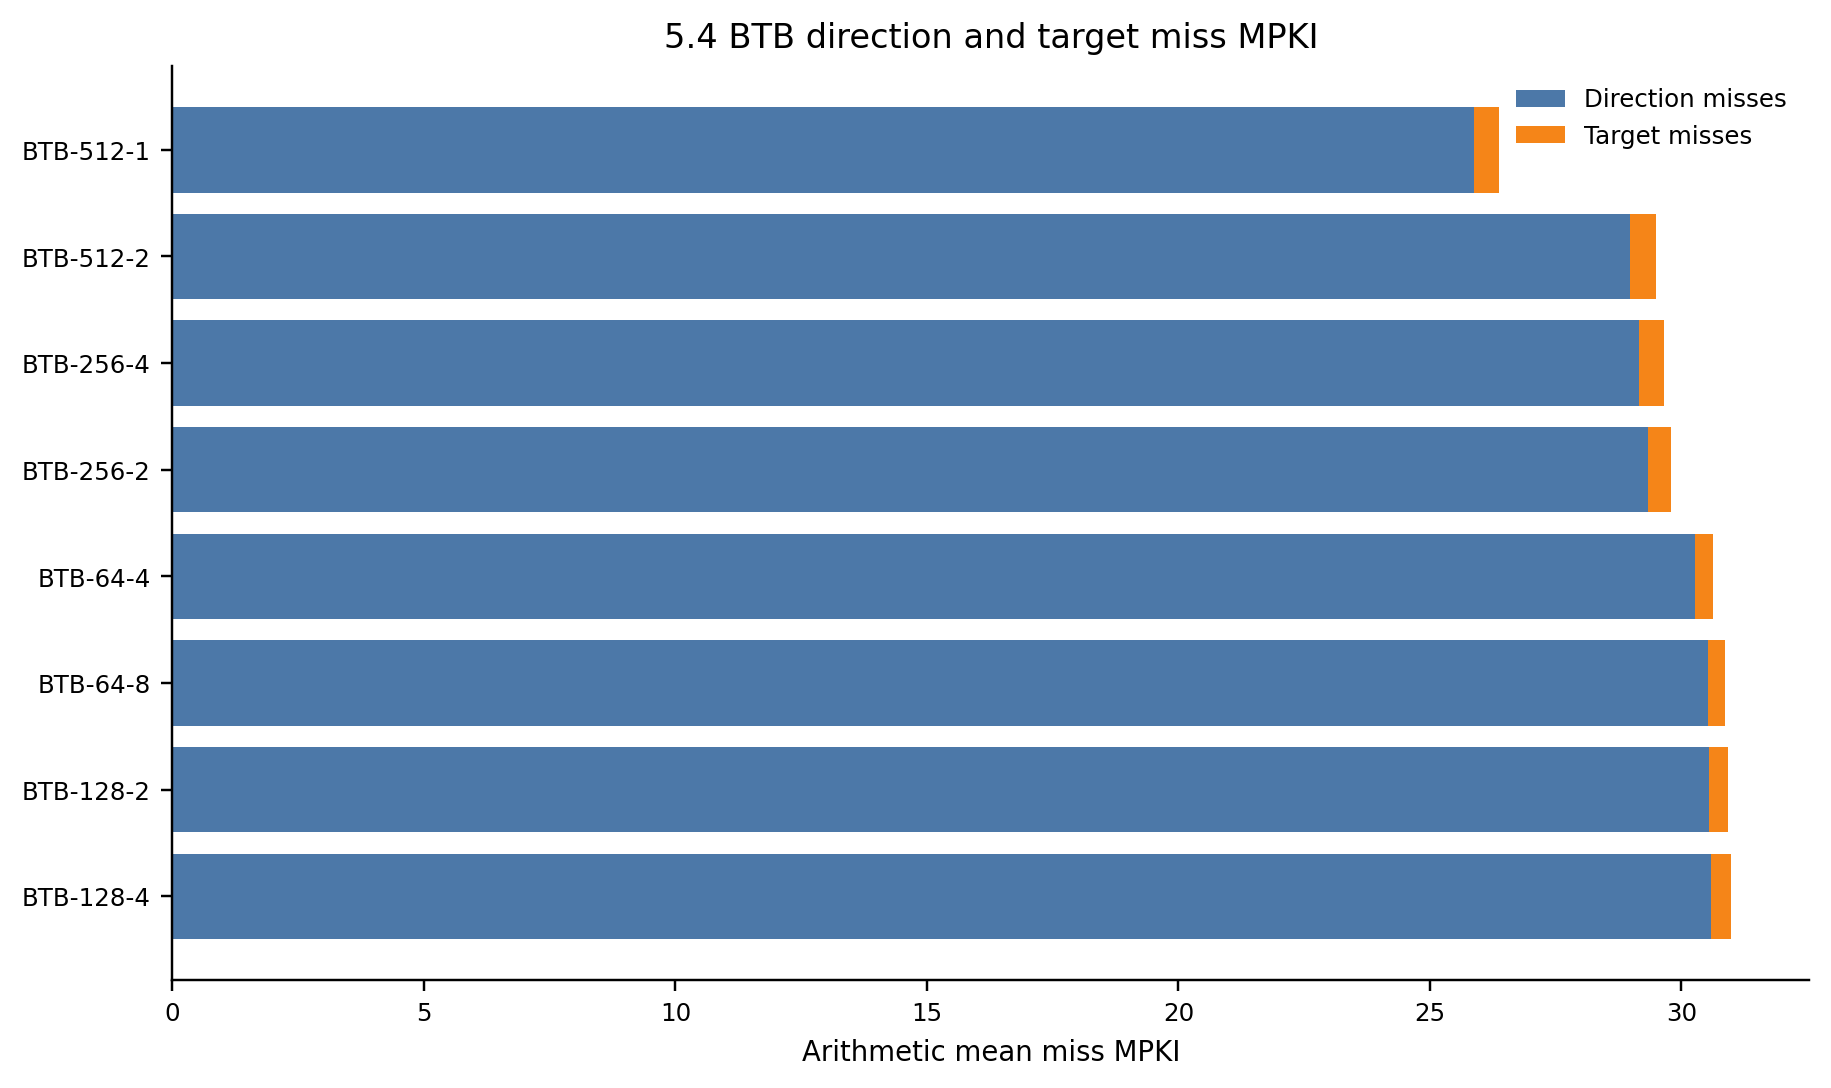
\includegraphics[width=0.86\linewidth]{5_4_btb_total_miss_mpki.png}
    \caption{Τιμές direction και target miss MPKI για τις οργανώσεις BTB.}
    \label{fig:btb_total}
\end{figure}

\begin{figure}[htbp]
    \centering
    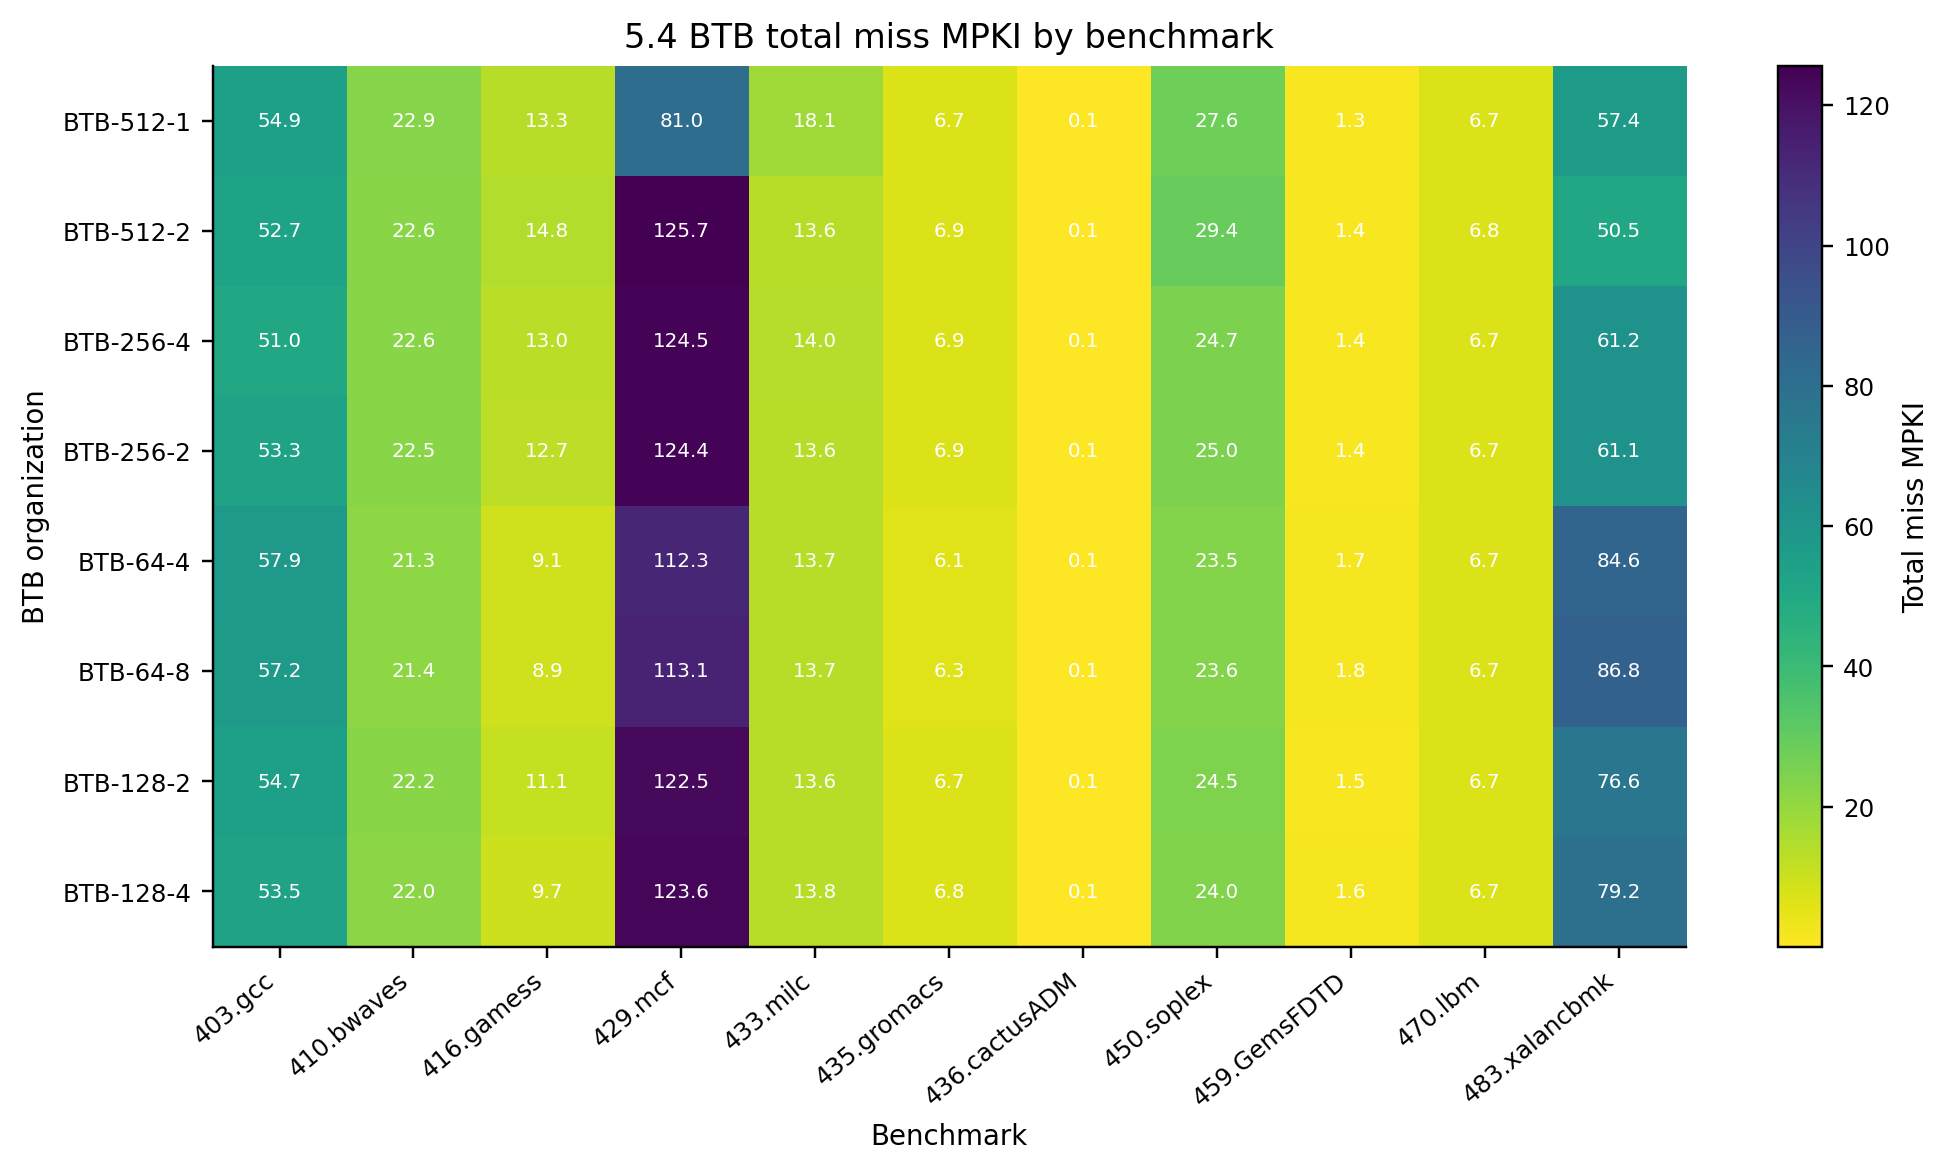
\includegraphics[width=0.98\linewidth]{5_4_btb_by_benchmark.png}
    \caption{Το total BTB miss MPKI ανά benchmark και οργάνωση.}
    \label{fig:btb_by_benchmark}
\end{figure}

\subsection{Αποτελέσματα και επιλογή}

Τα αποτελέσματα δείχνουν ότι τα target misses είναι πολύ λιγότερα από τα direction misses. Για παράδειγμα, στον \texttt{BTB-512-1}, ο αριθμητικός μέσος direction miss rate είναι 23.12\%, ενώ ο αντίστοιχος target miss rate είναι μόλις 0.62\%. Άρα, στα συγκεκριμένα traces, η συνολική επίδοση του BTB καθορίζεται κυρίως από το αν η δομή μπορεί να αναγνωρίσει έγκαιρα τα taken branches και όχι τόσο από το αν αποθηκεύει λανθασμένα targets για branches που έχουν ήδη προβλεφθεί ως taken.

\begin{center}
\begin{tabular}{lrrrr}
\toprule
BTB & Sets & Mean total MPKI & Aggregate total MPKI & Mean target miss\% \\
\midrule
\texttt{BTB-512-1} & 512 & 26.370 & 18.926 & 0.621 \\
\texttt{BTB-512-2} & 256 & 29.499 & 18.510 & 0.571 \\
\texttt{BTB-256-4} & 64 & 29.646 & 19.838 & 0.568 \\
\texttt{BTB-256-2} & 128 & 29.798 & 19.766 & 0.594 \\
\texttt{BTB-64-4} & 16 & 30.629 & 22.167 & 0.635 \\
\texttt{BTB-64-8} & 8 & 30.868 & 22.570 & 0.603 \\
\texttt{BTB-128-2} & 64 & 30.925 & 21.700 & 0.570 \\
\texttt{BTB-128-4} & 32 & 30.990 & 21.926 & 0.590 \\
\bottomrule
\end{tabular}
\captionof{table}{Συνοπτικά αποτελέσματα BTB.}
\label{tab:btb}
\end{center}

Με βάση τον αριθμητικό μέσο του total miss MPKI, η καλύτερη οργάνωση είναι η \texttt{BTB-512-1}, με τιμή 26.370. Το \texttt{BTB-512-2} έχει ελαφρώς καλύτερο aggregate total MPKI, 18.510 έναντι 18.926, αλλά χειρότερο αριθμητικό μέσο. Αυτό δείχνει ότι η δεύτερη οργάνωση ευνοείται περισσότερο από τα benchmarks με μεγάλο βάρος σε δυναμικές εντολές, χωρίς όμως να είναι συνολικά πιο σταθερή επιλογή σε όλα τα benchmarks.

Η γενική τάση είναι ότι η αύξηση του συνολικού αριθμού entries αποδίδει περισσότερο από την αύξηση του associativity. Αυτό σημαίνει ότι το κυρίαρχο πρόβλημα στα συγκεκριμένα πειράματα είναι κυρίως το capacity και όχι τα καθαρά conflict misses. Επομένως, για την παρούσα άσκηση επιλέγεται το \texttt{BTB-512-1}: είναι η καλύτερη οργάνωση ως προς τον αριθμητικό μέσο, είναι απλή, άμεσα αντιστοιχισμένη δομή και προσφέρει την πιο ισορροπημένη συμπεριφορά στο σύνολο των benchmarks.

\FloatBarrier
\section{5.5 Μελέτη του RAS}

\subsection{Θεωρία και υλοποίηση}

Η \foreignlanguage{english}{Return Address Stack} (RAS) χρησιμοποιείται για την πρόβλεψη των targets των return instructions. Τα returns είναι ιδιαίτερη κατηγορία branches, επειδή η ίδια στατική εντολή return μπορεί να επιστρέψει σε διαφορετικές διευθύνσεις, ανάλογα με το από ποιο call site κλήθηκε η συνάρτηση. Για αυτόν τον λόγο, ένας απλός BTB δεν είναι πάντα κατάλληλος για returns.

Η RAS εκμεταλλεύεται τη LIFO φύση των κλήσεων συναρτήσεων. Σε κάθε call γίνεται push η διεύθυνση επιστροφής, ενώ σε κάθε return γίνεται pop και η τιμή που αφαιρείται από τη στοίβα συγκρίνεται με το πραγματικό target. Αν οι κλήσεις και οι επιστροφές είναι καλά φωλιασμένες, τότε ακόμη και μια σχετικά μικρή RAS μπορεί να πετύχει πολύ υψηλή ακρίβεια. Τα προβλήματα εμφανίζονται όταν το δυναμικό βάθος κλήσεων ξεπερνά το μέγεθος της στοίβας ή όταν υπάρχουν πιο σύνθετες ροές ελέγχου που παραβιάζουν την καθαρή LIFO συμπεριφορά.

Η βασική μετρική είναι:
\[
    \text{RAS miss rate} =
    \frac{\text{incorrect returns}}{\text{correct returns} + \text{incorrect returns}} \cdot 100\%.
\]
Παράλληλα, υπολογίστηκε και RAS miss MPKI, ώστε να εκφραστεί η επίδραση των λανθασμένων προβλέψεων επιστροφής ως προς το συνολικό πλήθος εκτελεσμένων εντολών.

\begin{figure}[htbp]
    \centering
    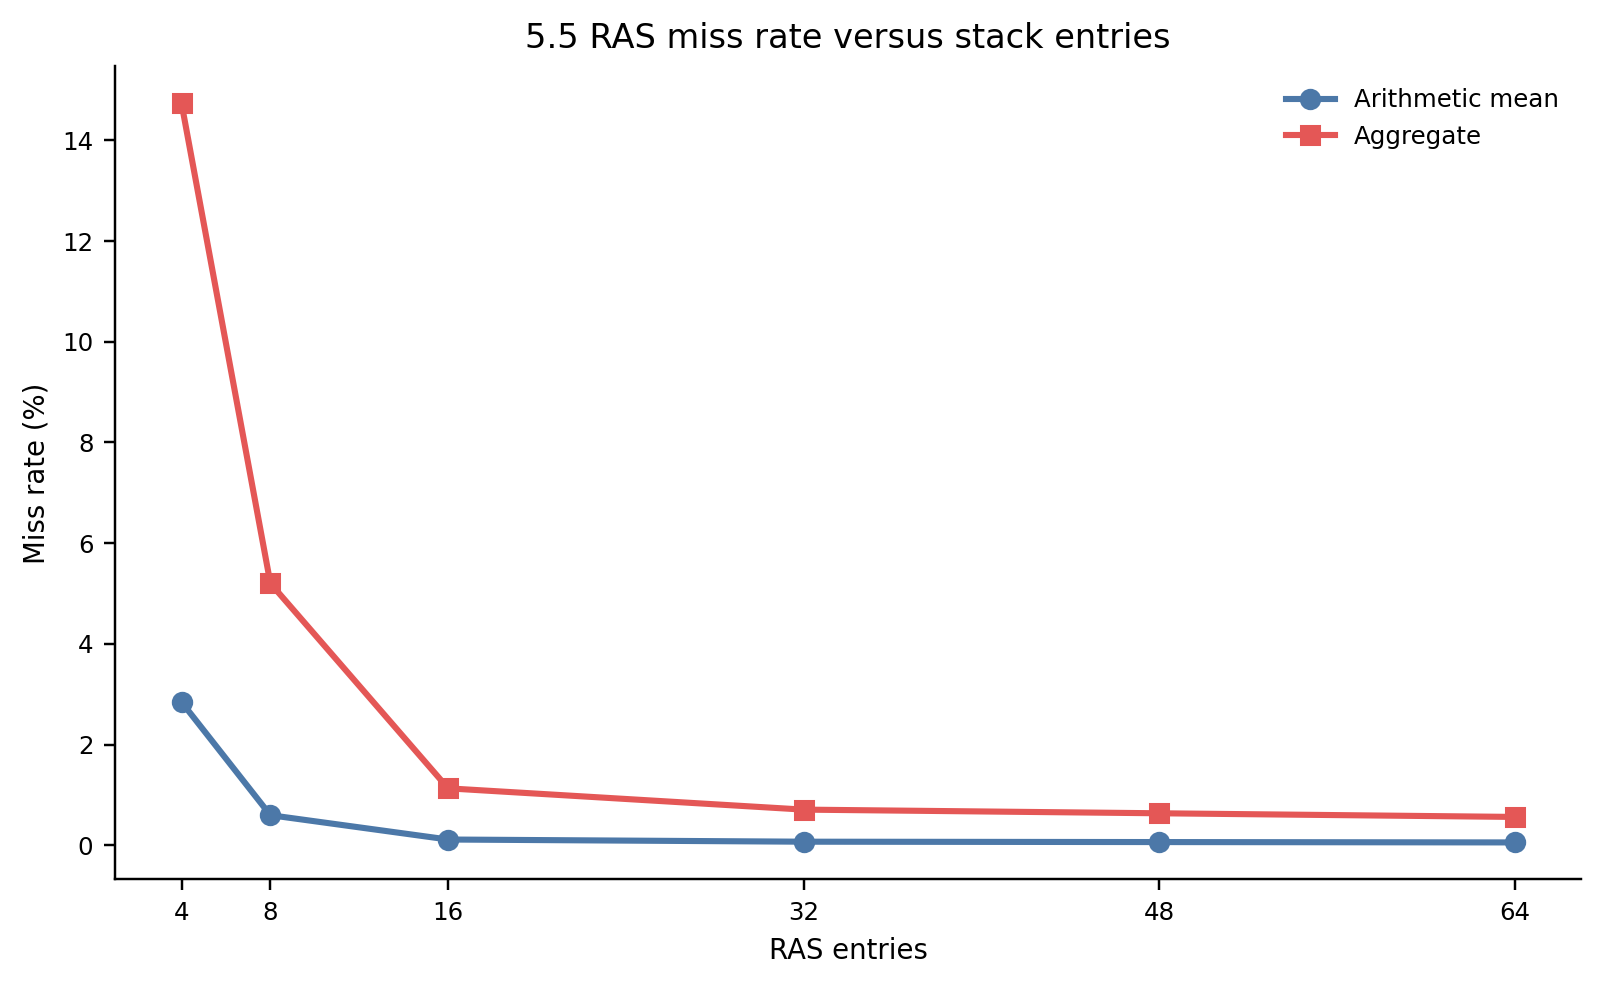
\includegraphics[width=0.78\linewidth]{5_5_ras_miss_rate.png}
    \caption{Ποσοστό αστοχίας RAS για διαφορετικά μεγέθη.}
    \label{fig:ras_miss_rate}
\end{figure}

\begin{figure}[htbp]
    \centering
    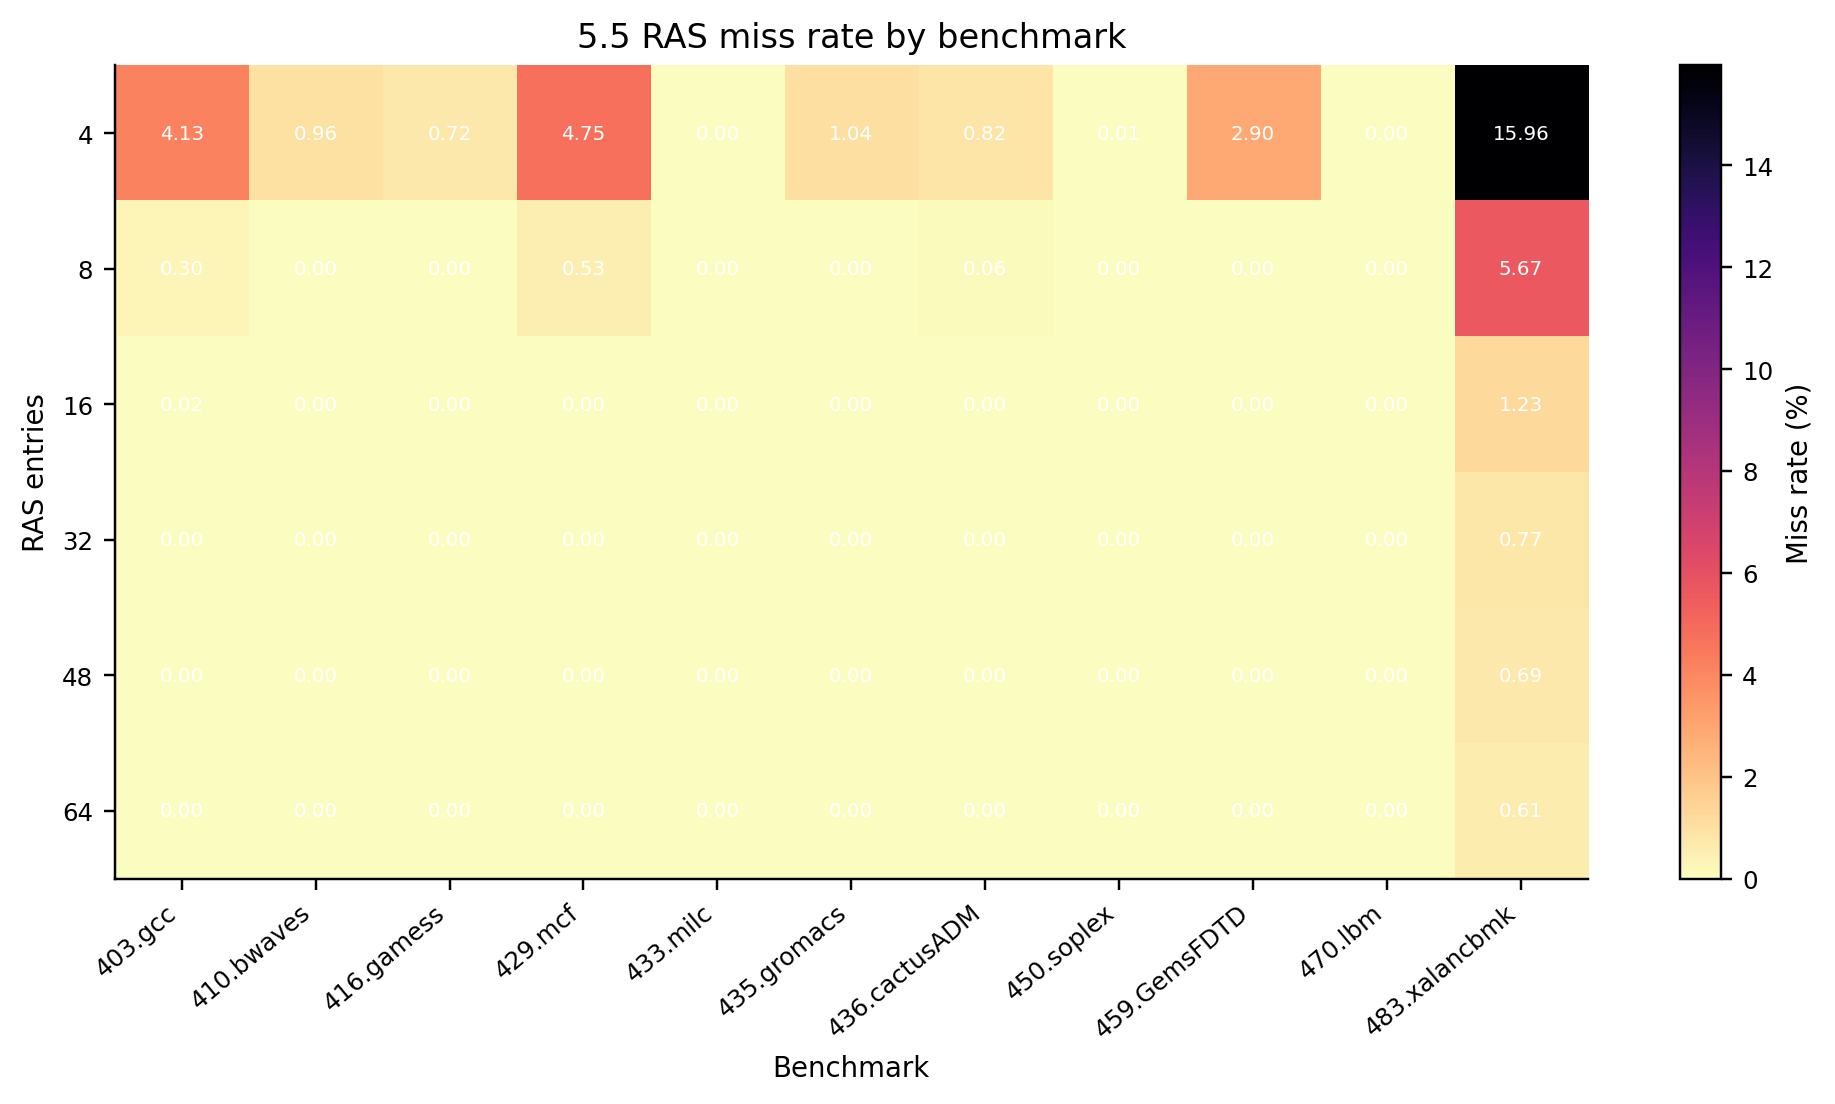
\includegraphics[width=0.95\linewidth]{5_5_ras_by_benchmark.png}
    \caption{Το RAS miss MPKI ανά benchmark και μέγεθος RAS.}
    \label{fig:ras_by_benchmark}
\end{figure}

\subsection{Αποτελέσματα και επιλογή}

\begin{center}
\begin{tabular}{rrrrr}
\toprule
Entries & Mean miss\% & Aggregate miss\% & Mean MPKI & Aggregate MPKI \\
\midrule
4 & 2.845 & 14.739 & 0.777 & 1.149 \\
8 & 0.597 & 5.203 & 0.254 & 0.405 \\
16 & 0.114 & 1.130 & 0.054 & 0.088 \\
32 & 0.070 & 0.707 & 0.034 & 0.055 \\
48 & 0.063 & 0.635 & 0.030 & 0.049 \\
64 & 0.056 & 0.562 & 0.027 & 0.044 \\
\bottomrule
\end{tabular}
\captionof{table}{Συνοπτικά αποτελέσματα RAS.}
\label{tab:ras}
\end{center}

Τα αποτελέσματα του Πίνακα~\ref{tab:ras} δείχνουν ότι η αύξηση του μεγέθους της RAS από 4 σε 16 entries μειώνει δραστικά τις αστοχίες. Ο αριθμητικός μέσος του miss rate πέφτει από 2.845\% σε 0.114\%, ενώ το mean MPKI από 0.777 σε 0.054. Άρα, τα 4 entries δεν αρκούν για να καλύψουν το δυναμικό βάθος κλήσεων των benchmarks, ενώ τα 16 entries καλύπτουν ήδη το μεγαλύτερο μέρος των περιπτώσεων.

Μετά τα 32 entries, η καμπύλη σχεδόν κορέννυται. Από 32 σε 64 entries, ο αριθμητικός μέσος του miss rate μειώνεται μόνο από 0.070\% σε 0.056\%, ενώ το mean MPKI από 0.034 σε 0.027. Η βελτίωση υπάρχει, αλλά είναι μικρή σε σχέση με τον διπλασιασμό του μεγέθους.

Αν το μοναδικό κριτήριο ήταν η ελάχιστη τιμή αστοχίας, τότε η RAS των 64 entries θα ήταν η καλύτερη επιλογή. Ωστόσο, από αρχιτεκτονική σκοπιά, η RAS των 32 entries είναι πιο ισορροπημένη. Βρίσκεται πρακτικά στο γόνατο της καμπύλης, προσφέρει πολύ χαμηλό miss MPKI και έχει μισό μέγεθος σε σχέση με τα 64 entries. Η επιλογή αυτή συμφωνεί με τη θεωρία της RAS: μόλις το μέγεθος της στοίβας καλύψει το συνηθισμένο βάθος δυναμικών κλήσεων, η περαιτέρω αύξηση προσφέρει μόνο οριακή βελτίωση.

\FloatBarrier
\section{5.6.1 Perceptrons}

\subsection{Θεωρητικό υπόβαθρο}

Οι perceptron predictors αποτελούν διαφορετική προσέγγιση από τους απλούς saturating counters. Αντί να αποθηκεύουν μόνο μια μικρή κατάσταση για κάθε branch, προσπαθούν να μάθουν συσχετίσεις ανάμεσα στο τρέχον branch και στο πρόσφατο global branch history. Με αυτόν τον τρόπο μπορούν να αξιοποιήσουν μοτίβα που εκτείνονται σε μεγαλύτερο βάθος ιστορίας.

Ένας perceptron predictor χρησιμοποιεί έναν πίνακα από \(M\) perceptrons και global history length \(n\). Κάθε perceptron έχει \(n+1\) βάρη:
\[
    w_0, w_1, \ldots, w_n,
\]
όπου το \(w_0\) είναι bias. Τα τελευταία \(n\) branch outcomes κωδικοποιούνται ως:
\[
    x_i =
    \begin{cases}
    -1, & \text{αν το branch ήταν not-taken},\\
    1, & \text{αν το branch ήταν taken}.
    \end{cases}
\]
Η έξοδος του perceptron είναι:
\[
    y = w_0 + \sum_{i=1}^{n} x_i w_i.
\]
Αν \(y \geq 0\), η πρόβλεψη είναι taken, ενώ αν \(y < 0\), η πρόβλεψη είναι not-taken.

Η εκπαίδευση γίνεται όταν η πρόβλεψη είναι λανθασμένη ή όταν είναι σωστή αλλά με μικρή εμπιστοσύνη:
\[
    |y| \leq \theta, \qquad
    \theta = \left\lfloor 1.93n + 14 \right\rfloor.
\]
Στην υλοποίηση της άσκησης, τα βάρη περιορίστηκαν στο διάστημα \([-\theta,\theta]\), ώστε ο υπολογισμός του κόστους hardware στο επόμενο ερώτημα να είναι συνεπής με το πλήθος των bits ανά βάρος.

Η βασική διαφορά από ένα PHT με 2-bit counters είναι ότι ο perceptron λειτουργεί ως γραμμικός ταξινομητής πάνω στο global history. Αυτό του επιτρέπει να μάθει μακρινές συσχετίσεις μεταξύ branches, με κόστος όμως μεγαλύτερο αποθηκευτικό χώρο και περισσότερη υπολογιστική πολυπλοκότητα, αφού απαιτείται υπολογισμός dot product σε κάθε πρόβλεψη.

\begin{figure}[htbp]
    \centering
    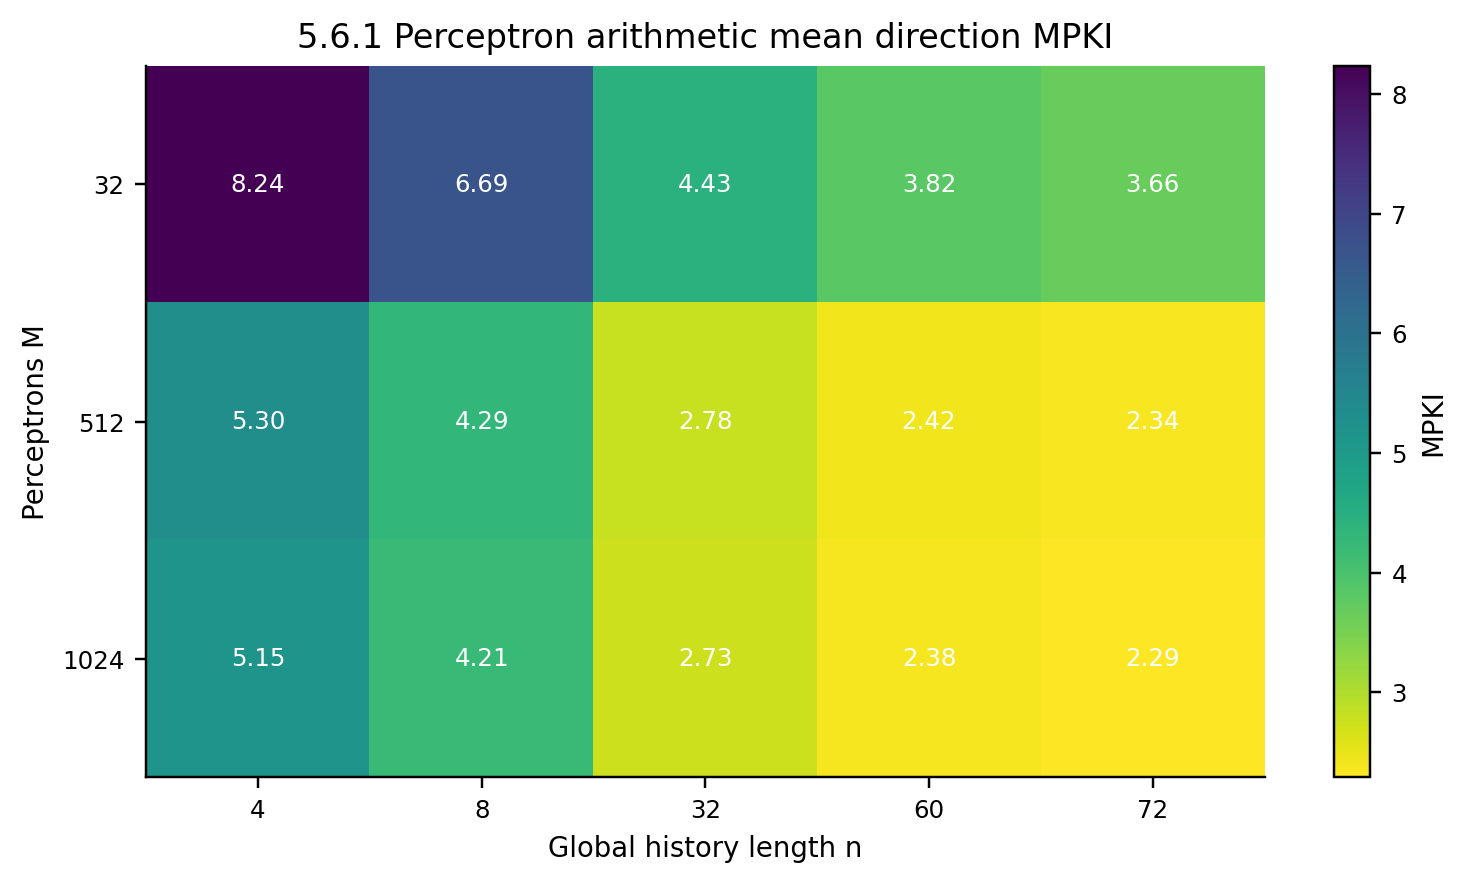
\includegraphics[width=0.72\linewidth]{5_6_1_perceptron_heatmap.png}
    \caption{Αριθμητικός μέσος του direction MPKI για τα απαιτούμενα ζεύγη \(M,n\).}
    \label{fig:perceptron_heatmap}
\end{figure}

\subsection{Σχολιασμός αποτελεσμάτων}

Το Σχήμα~\ref{fig:perceptron_heatmap} δείχνει ότι το global history length \(n\) είναι ο σημαντικότερος παράγοντας για την επίδοση. Η μέση τιμή του MPKI ανά \(n\), συνυπολογίζοντας τις τρεις τιμές του \(M\), μειώνεται από 6.229 για \(n=4\) σε 2.763 για \(n=72\). Άρα, στα συγκεκριμένα benchmarks υπάρχουν αξιοποιήσιμες συσχετίσεις που εκτείνονται αρκετά πίσω στο ιστορικό εκτέλεσης.

Η αύξηση του \(M\) βοηθά επίσης, επειδή μειώνει το aliasing μεταξύ διαφορετικών branch PCs που χαρτογραφούνται στον ίδιο perceptron. Ωστόσο, το όφελος από την αύξηση του \(M\) από 512 σε 1024 είναι μικρότερο από το όφελος που δίνει η αύξηση του \(n\). Αυτό είναι αναμενόμενο: περισσότερα perceptrons μειώνουν τις συγκρούσεις, αλλά μεγαλύτερο history length προσθέτει ουσιαστικά νέα πληροφορία για τη συσχέτιση μεταξύ branches.

\begin{center}
\begin{tabular}{lrrrr}
\toprule
Predictor & \(M\) & \(n\) & Mean MPKI & Aggregate MPKI \\
\midrule
\texttt{Perceptron-M1024-N72} & 1024 & 72 & 2.287 & 1.333 \\
\texttt{Perceptron-M512-N72} & 512 & 72 & 2.336 & 1.339 \\
\texttt{Perceptron-M1024-N60} & 1024 & 60 & 2.375 & 1.472 \\
\texttt{Perceptron-M512-N60} & 512 & 60 & 2.424 & 1.477 \\
\texttt{Perceptron-M1024-N32} & 1024 & 32 & 2.732 & 2.025 \\
\bottomrule
\end{tabular}
\captionof{table}{Καλύτερες διαμορφώσεις perceptron στο 5.6.1.}
\label{tab:perceptron_best}
\end{center}

Η καλύτερη διαμόρφωση του ερωτήματος είναι η \texttt{Perceptron-M1024-N72}, με mean MPKI 2.287 και aggregate MPKI 1.333. Η επίδοση αυτή είναι αισθητά καλύτερη από τους απλούς n-bit predictors, γεγονός που δείχνει τη δύναμη του μεγάλου global history όταν οι συσχετίσεις των branches είναι σε μεγάλο βαθμό γραμμικά αξιοποιήσιμες.

Παρ' όλα αυτά, η συγκεκριμένη διαμόρφωση δεν είναι άμεσα συγκρίσιμη με τους predictors του 5.6.2, επειδή απαιτεί πολύ μεγαλύτερο κόστος hardware από το περίπου 32K-bit budget. Για αυτόν τον λόγο, στο επόμενο ερώτημα χρησιμοποιούνται μικρότερες διαμορφώσεις perceptron, οι οποίες έχουν κόστος κοντά στα 32K bits.

\FloatBarrier
\section{5.6.2 Σύγκριση διαφορετικών μηχανισμών πρόβλεψης}

\subsection{Υλοποίηση και επιλογές hardware}

Στο ερώτημα 5.6.2 συγκρίθηκαν 18 διαφορετικοί predictors. Η σύγκριση αυτή είναι το πιο ολοκληρωμένο μέρος της άσκησης, επειδή περιλαμβάνει από πολύ απλούς static predictors μέχρι πιο σύνθετους hybrid και perceptron-based μηχανισμούς. Έτσι, εξετάζονται οι βασικές οικογένειες τεχνικών πρόβλεψης: στατική πρόβλεψη, απλή δυναμική πρόβλεψη, local history, global history, perceptrons και υβριδικοί μηχανισμοί επιλογής.

Οι static predictors χρησιμοποιούνται ως baselines. Ο \texttt{Static-AlwaysTaken} προβλέπει πάντα taken, ενώ ο \texttt{Static-BTFNT} προβλέπει taken για backward branches και not-taken για forward branches. Ο κανόνας BTFNT είναι πιο λογικός για loops, επειδή τα backward branches αντιστοιχούν συχνά σε επαναλήψεις που εκτελούνται πολλές φορές.

Για τους local-history predictors κρατήθηκε σταθερό:
\[
    \text{PHT} = 8192 \cdot 2 = 16K \text{ bits}.
\]
Το υπόλοιπο budget χρησιμοποιήθηκε για το BHT. Έτσι, για συνολικό κόστος 32K bits επιλέχθηκαν οι διαμορφώσεις:
\[
    (X,Z) = (2048,8), (4096,4), (8192,2).
\]
Οι local-history predictors είναι χρήσιμοι όταν ένα συγκεκριμένο static branch έχει δικό του επαναλαμβανόμενο μοτίβο.

Για τους global-history predictors αγνοήθηκε το μικρό κόστος του BHR, όπως επιτρέπει η εκφώνηση. Επομένως:
\[
    Z \cdot 2 = 32K \Rightarrow Z = 16K \text{ PHT entries}.
\]
Συγκρίθηκαν BHR μήκη 4, 8 και 12. Οι global-history predictors είναι κατάλληλοι όταν η συμπεριφορά ενός branch εξαρτάται από προηγούμενα branches, δηλαδή όταν υπάρχει inter-branch correlation.

Για τα perceptrons χρησιμοποιήθηκε ο τύπος:
\[
    \text{bits} = M(n+1)(1+\lfloor \log_2\theta \rfloor),
    \qquad
    \theta = \lfloor 1.93n + 14 \rfloor.
\]
Οι τρεις επιλογές κοντά στα 32K bits ήταν:
\[
    \texttt{M728-N8}: 32760 \text{ bits}, \quad
    \texttt{M141-N32}: 32571 \text{ bits}, \quad
    \texttt{M56-N72}: 32704 \text{ bits}.
\]
Με αυτές τις επιλογές φαίνεται καθαρά το trade-off μεταξύ πλήθους perceptrons και μήκους ιστορίας. Πολλά perceptrons μειώνουν το aliasing, ενώ μεγάλο \(n\) επιτρέπει μάθηση μακρύτερων συσχετίσεων.

Ο \texttt{Alpha21264} υλοποιήθηκε ως hybrid predictor με local history table 1024 entries των 10 bits, local PHT 1024 entries των 3 bits, global PHT 4096 entries των 2 bits και choice PHT 4096 entries των 2 bits. Το συνολικό κόστος είναι 29696 bits. Η σημαντική ιδέα είναι ότι ο choice predictor δεν προβλέπει απευθείας το branch, αλλά μαθαίνει αν για το συγκεκριμένο branch είναι προτιμότερη η local ή η global συνιστώσα.

Τέλος, στους tournament predictors αγνοήθηκε το κόστος του meta-predictor, όπως ζητείται. Περίπου 16K bits δόθηκαν σε κάθε συνιστώσα \(P_0\) και \(P_1\). Η λογική των tournament predictors είναι παρόμοια με αυτή των hybrid predictors: αντί να βασίζονται σε μία μόνο υπόθεση για τη συμπεριφορά όλων των branches, επιτρέπουν σε διαφορετικούς predictors να είναι υπεύθυνοι για διαφορετικά μοτίβα.

\begin{figure}[htbp]
    \centering
    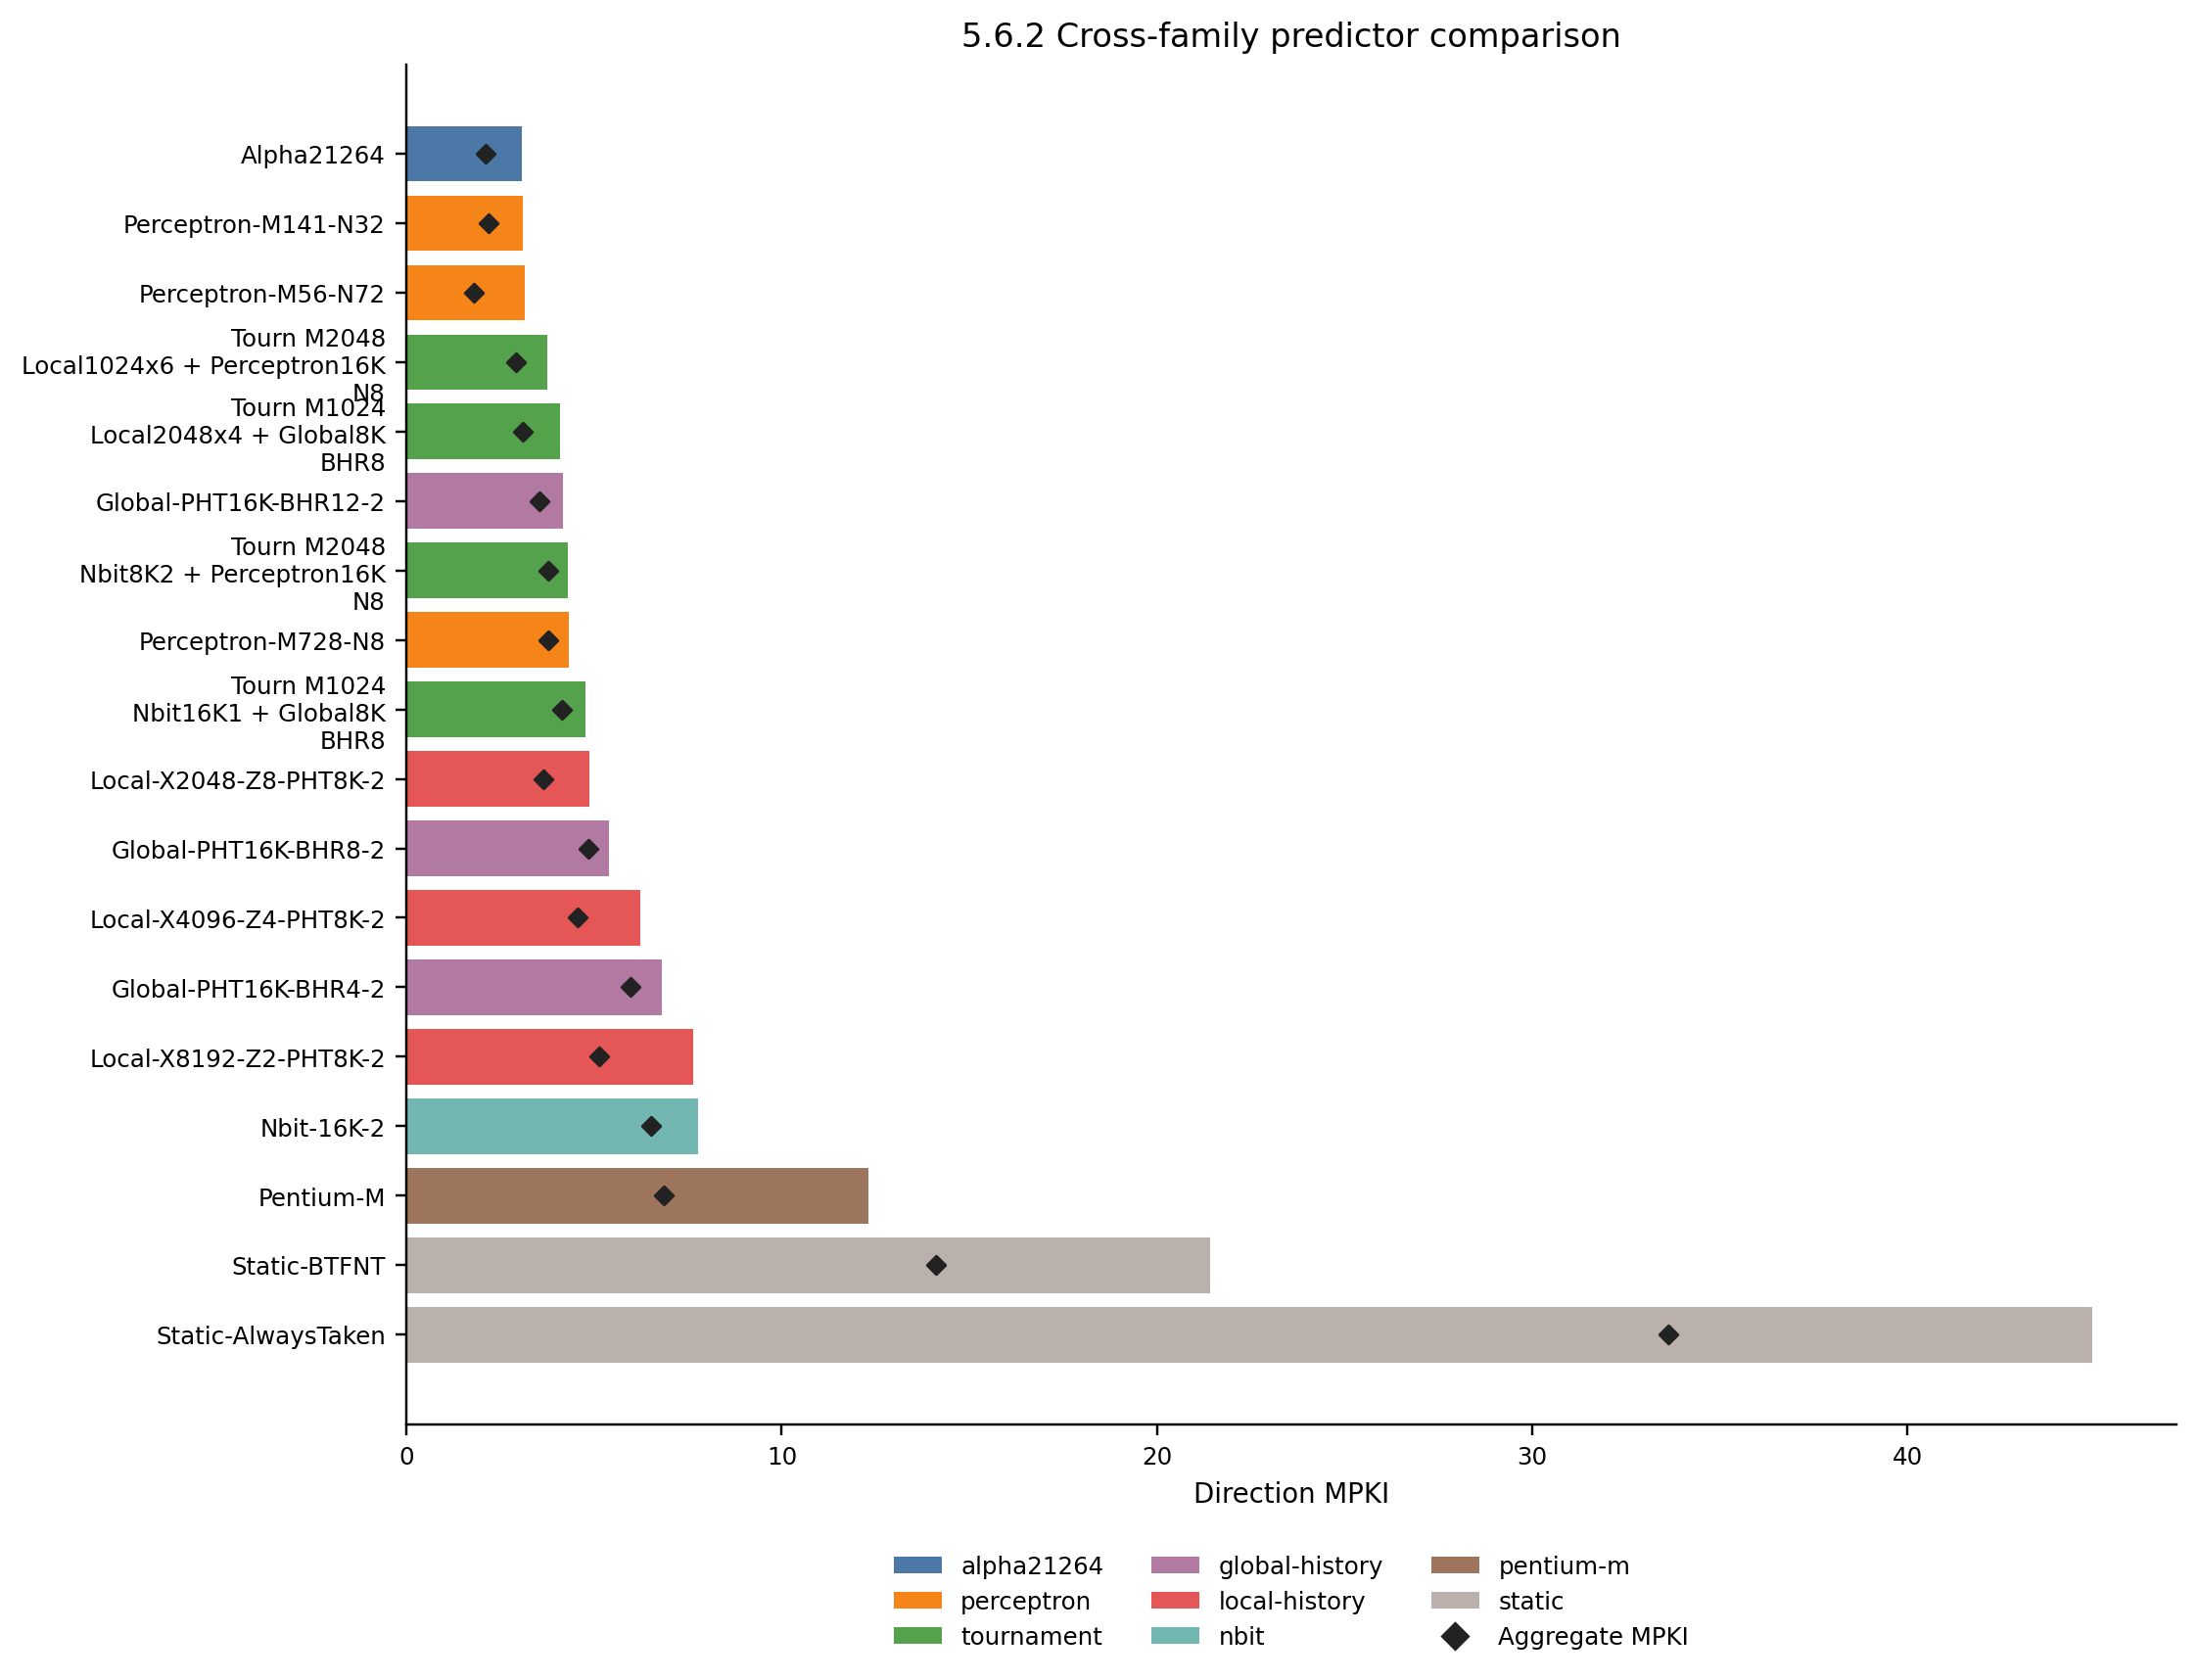
\includegraphics[width=0.92\linewidth]{5_6_2_predictor_comparison.png}
    \caption{Σύγκριση των 18 predictors του 5.6.2. Οι μπάρες δείχνουν τον αριθμητικό μέσο του MPKI και τα μαύρα σημεία δείχνουν το aggregate MPKI.}
    \label{fig:predictor_comparison}
\end{figure}

\begin{figure}[htbp]
    \centering
    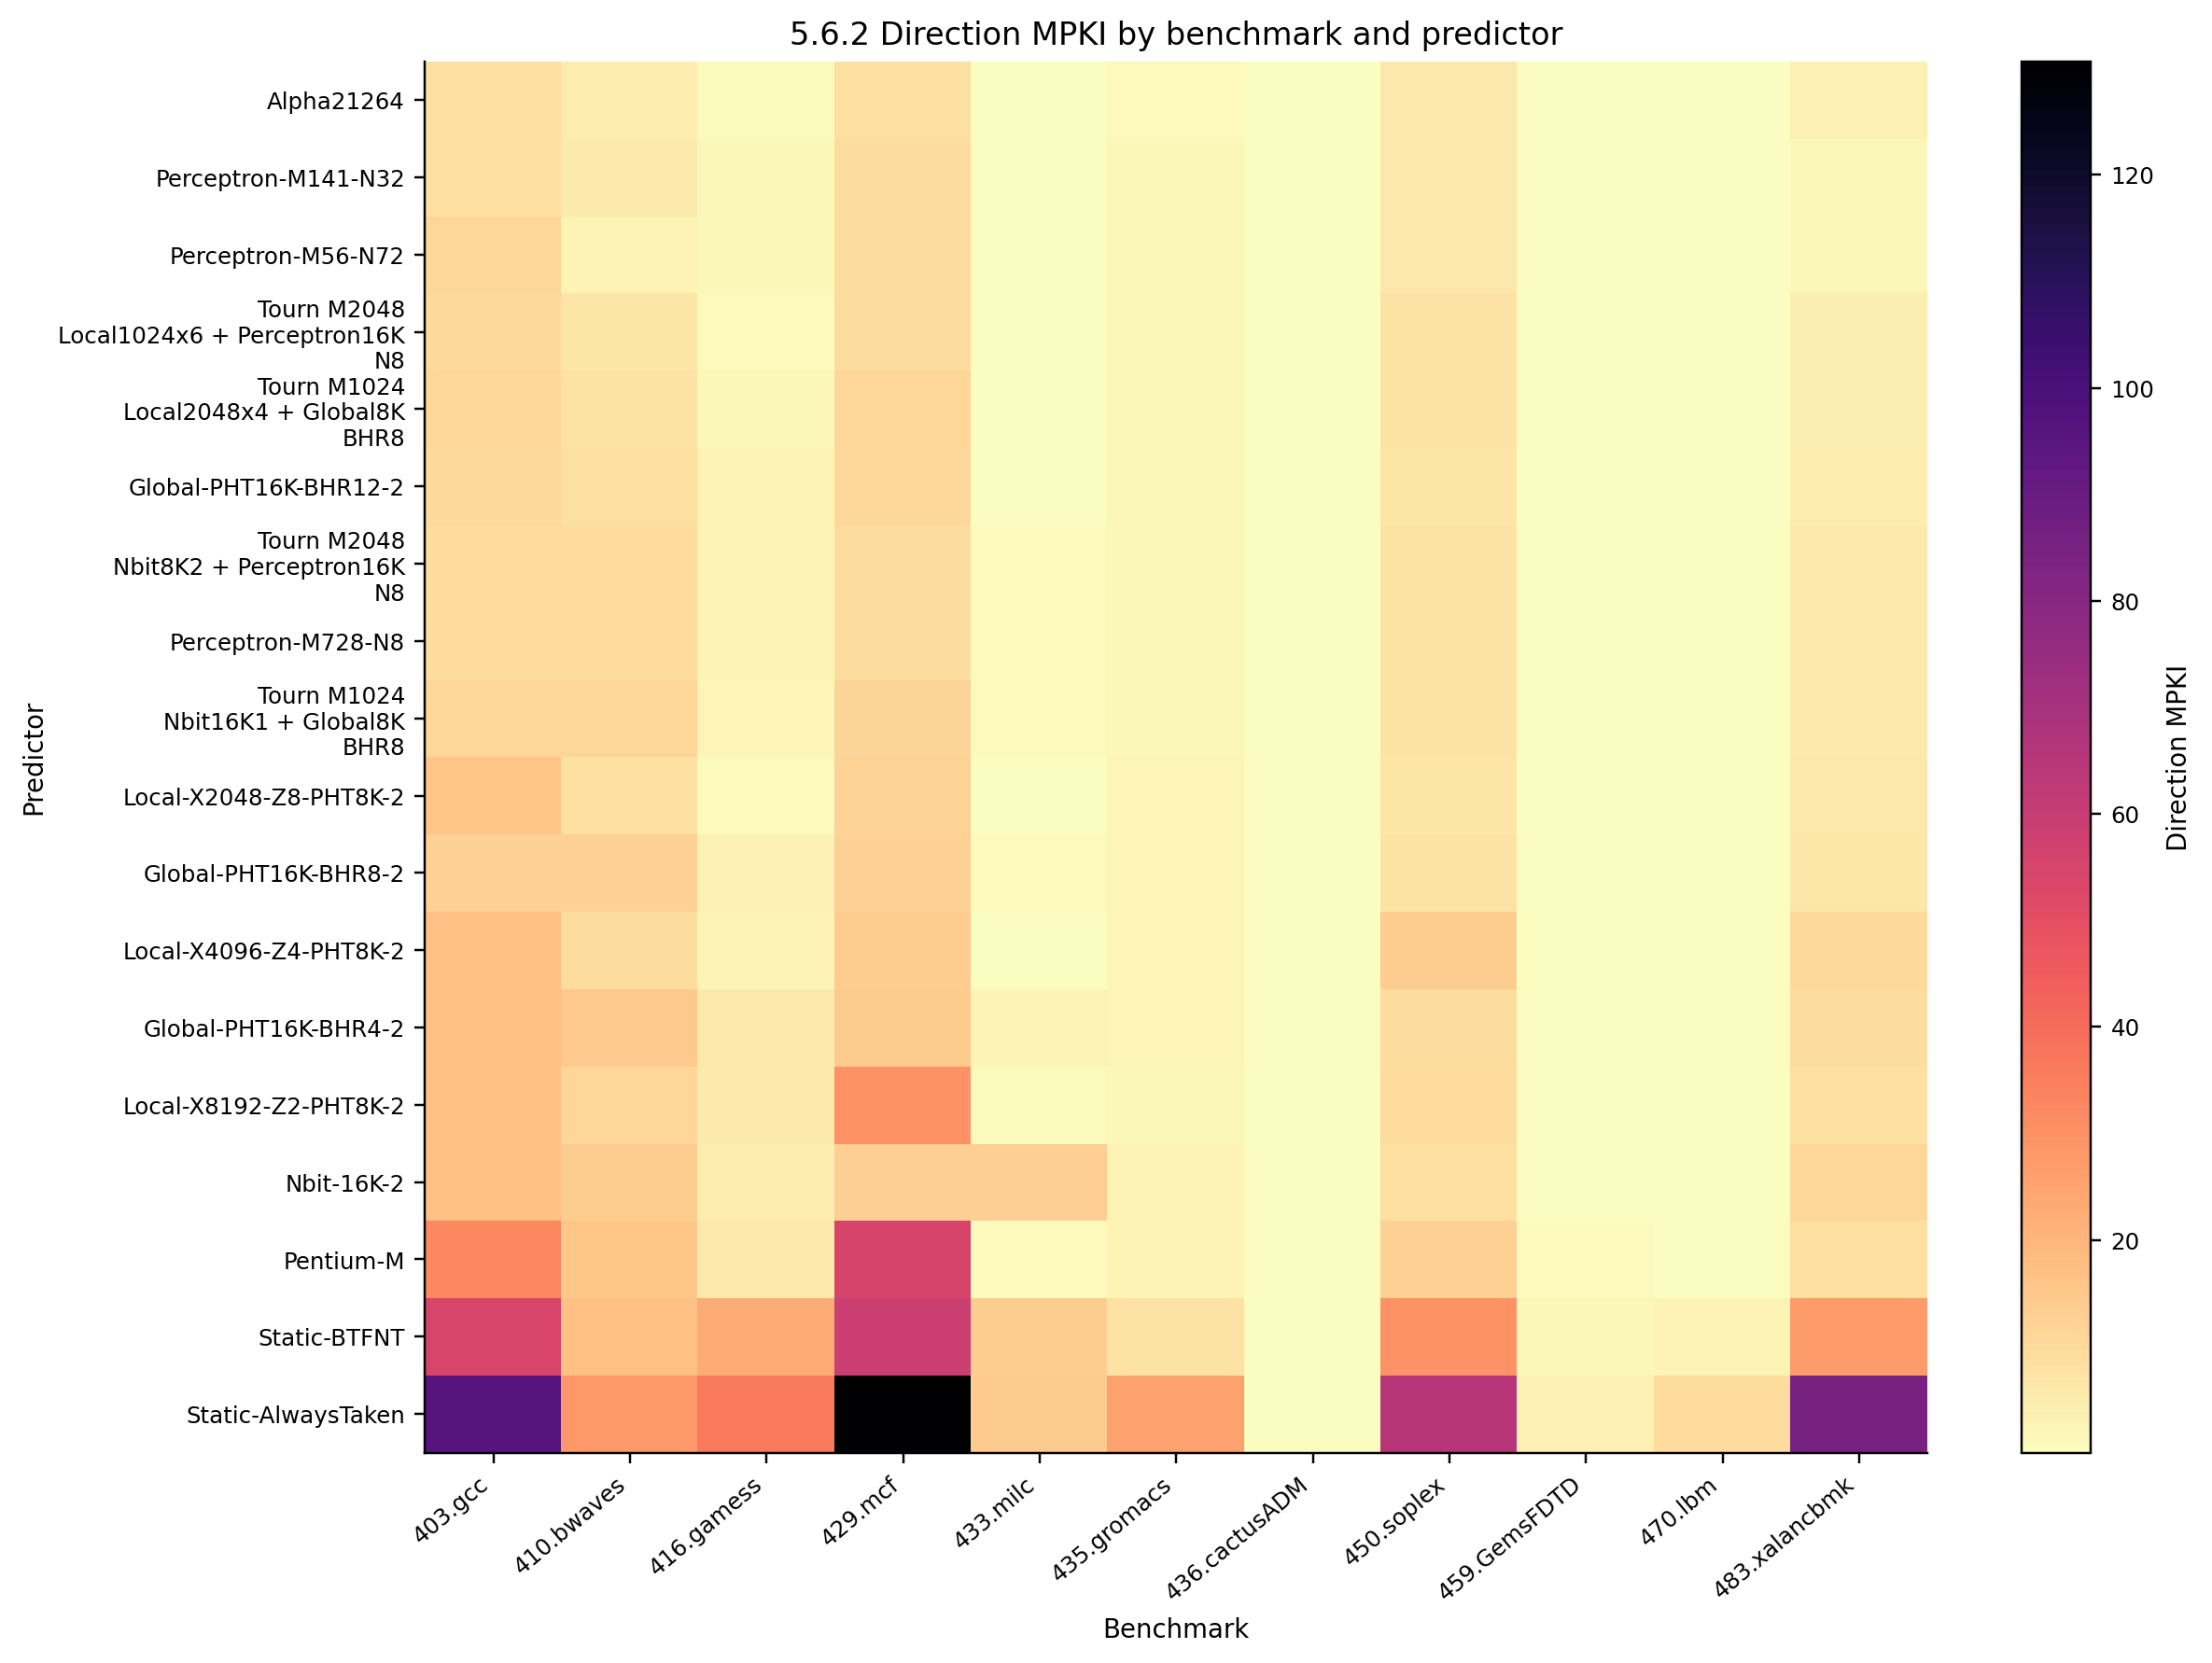
\includegraphics[width=0.98\linewidth]{5_6_2_predictor_by_benchmark.png}
    \caption{Το direction MPKI ανά benchmark για τους predictors του 5.6.2.}
    \label{fig:predictor_by_benchmark}
\end{figure}

\subsection{Αποτελέσματα και τελική επιλογή}

\begin{center}
\resizebox{\linewidth}{!}{%
\begin{tabular}{llrrr}
\toprule
Predictor & Family & Bits & Mean MPKI & Aggregate MPKI \\
\midrule
\texttt{Alpha21264} & alpha21264 & 29696 & 3.071 & 2.119 \\
\texttt{Perceptron-M141-N32} & perceptron & 32571 & 3.088 & 2.186 \\
\texttt{Perceptron-M56-N72} & perceptron & 32704 & 3.140 & 1.788 \\
\texttt{Tournament-M2048-Local1024x6-Perceptron16K-N8} & tournament & 30716 & 3.743 & 2.922 \\
\texttt{Tournament-M1024-Local2048x4-Global8K-BHR8} & tournament & 32768 & 4.091 & 3.102 \\
\texttt{Global-PHT16K-BHR12-2} & global-history & 32768 & 4.181 & 3.555 \\
\texttt{Perceptron-M728-N8} & perceptron & 32760 & 4.314 & 3.768 \\
\texttt{Nbit-16K-2} & nbit & 32768 & 7.770 & 6.505 \\
\texttt{Static-BTFNT} & static & 0 & 21.430 & 14.108 \\
\texttt{Static-AlwaysTaken} & static & 0 & 44.920 & 33.623 \\
\bottomrule
\end{tabular}%
}
\captionof{table}{Επιλεγμένες γραμμές από τη συνολική σύγκριση των 18 predictors.}
\label{tab:predictor_comparison}
\end{center}

Η συνολική κατάταξη είναι αρκετά καθαρή. Οι static predictors είναι χρήσιμοι ως σημεία αναφοράς, αλλά απέχουν σημαντικά από τους dynamic predictors. Ο \texttt{Static-BTFNT} είναι πολύ καλύτερος από τον \texttt{Static-AlwaysTaken}, επειδή αξιοποιεί τη συχνή συμπεριφορά των loops, όμως παραμένει ένας απλός κανόνας χωρίς προσαρμογή στη δυναμική συμπεριφορά κάθε branch.

Ο απλός \texttt{Nbit-16K-2} βελτιώνει σημαντικά τους static predictors, αλλά υστερεί έναντι των μηχανισμών που αξιοποιούν ιστορικό. Αυτό είναι αναμενόμενο, επειδή ο 2-bit predictor θυμάται μόνο την πρόσφατη τάση κάθε branch και δεν μπορεί να μάθει πιο σύνθετα μοτίβα.

Οι local-history και global-history predictors μειώνουν σημαντικά το MPKI. Στην κατηγορία των global-history predictors, η καλύτερη διαμόρφωση είναι η \texttt{Global-PHT16K-BHR12-2}, με mean MPKI 4.181. Το αποτέλεσμα αυτό δείχνει ότι υπάρχει αξιοποιήσιμη συσχέτιση μεταξύ διαφορετικών branches. Αν η συμπεριφορά κάθε branch ήταν πλήρως ανεξάρτητη, τότε το global history δεν θα προσέφερε τόσο μεγάλη βελτίωση.

Οι tournament predictors βελτιώνουν περαιτέρω την εικόνα, ειδικά όταν συνδυάζουν local history με perceptron συνιστώσα. Η καλύτερη tournament διαμόρφωση, \texttt{Tournament-M2048-Local1024x6-Perceptron16K-N8}, πετυχαίνει mean MPKI 3.743. Ωστόσο, δεν φτάνει τους τρεις καλύτερους predictors της συνολικής σύγκρισης.

Οι τρεις κορυφαίες διαμορφώσεις με βάση τον αριθμητικό μέσο είναι:
\[
    \texttt{Alpha21264}, \quad
    \texttt{Perceptron-M141-N32}, \quad
    \texttt{Perceptron-M56-N72}.
\]
Ο \texttt{Alpha21264} έχει το καλύτερο mean MPKI, 3.071, και μικρότερο κόστος από τις δύο perceptron διαμορφώσεις. Ο \texttt{Perceptron-M141-N32} είναι πρακτικά ισοδύναμος σε αριθμητικό μέσο, με 3.088, ενώ ο \texttt{Perceptron-M56-N72} έχει την καλύτερη aggregate τιμή, 1.788. Αυτό σημαίνει ότι ο μεγάλης ιστορίας perceptron αποδίδει ιδιαίτερα καλά στα benchmarks που έχουν μεγάλο βάρος σε δυναμικές εντολές.

Ως τελική επιλογή μετά το 5.6.2 προκρίνεται ο \texttt{Alpha21264}. Ο λόγος δεν είναι μόνο ότι έχει το μικρότερο mean MPKI, αλλά και ότι αποτελεί πιο ισορροπημένη αρχιτεκτονική λύση. Συνδυάζει local και global πληροφορία, χρησιμοποιεί choice predictor για να επιλέγει δυναμικά την καταλληλότερη συνιστώσα, έχει κόστος 29696 bits και δεν απαιτεί dot product πολλών βαρών σε κάθε πρόβλεψη, όπως οι perceptrons. Επομένως, προσφέρει πολύ καλή ακρίβεια με πιο πρακτική μικροαρχιτεκτονική πολυπλοκότητα.

\FloatBarrier
\section{5.7 Ακρίβεια προσομοιώσεων με \texttt{ref} inputs}

\subsection{Επιλογή μηχανισμών πρόβλεψης για έλεγχο}

Το ερώτημα 5.7 εξετάζει αν τα συμπεράσματα που προέκυψαν από τα \texttt{train} inputs διατηρούνται και στα \texttt{ref} inputs. Τα \texttt{ref} inputs είναι μεγαλύτερα και γενικά πιο αντιπροσωπευτικά, άρα αποτελούν πιο αυστηρό έλεγχο για την αξιοπιστία της τελικής επιλογής.

Επιλέχθηκαν οι τρεις καλύτεροι predictors του 5.6.2 με βάση τον αριθμητικό μέσο του direction MPKI:
\[
    \texttt{Alpha21264}, \quad
    \texttt{Perceptron-M141-N32}, \quad
    \texttt{Perceptron-M56-N72}.
\]
Δεν επιλέχθηκαν οι πολύ μεγάλες perceptron διαμορφώσεις του 5.6.1, παρότι είχαν χαμηλότερο MPKI, επειδή ξεπερνούν σημαντικά το περίπου 32K-bit budget. Η σύγκριση του 5.7 πρέπει να παραμείνει δίκαιη ως προς το hardware κόστος.

\begin{figure}[htbp]
    \centering
    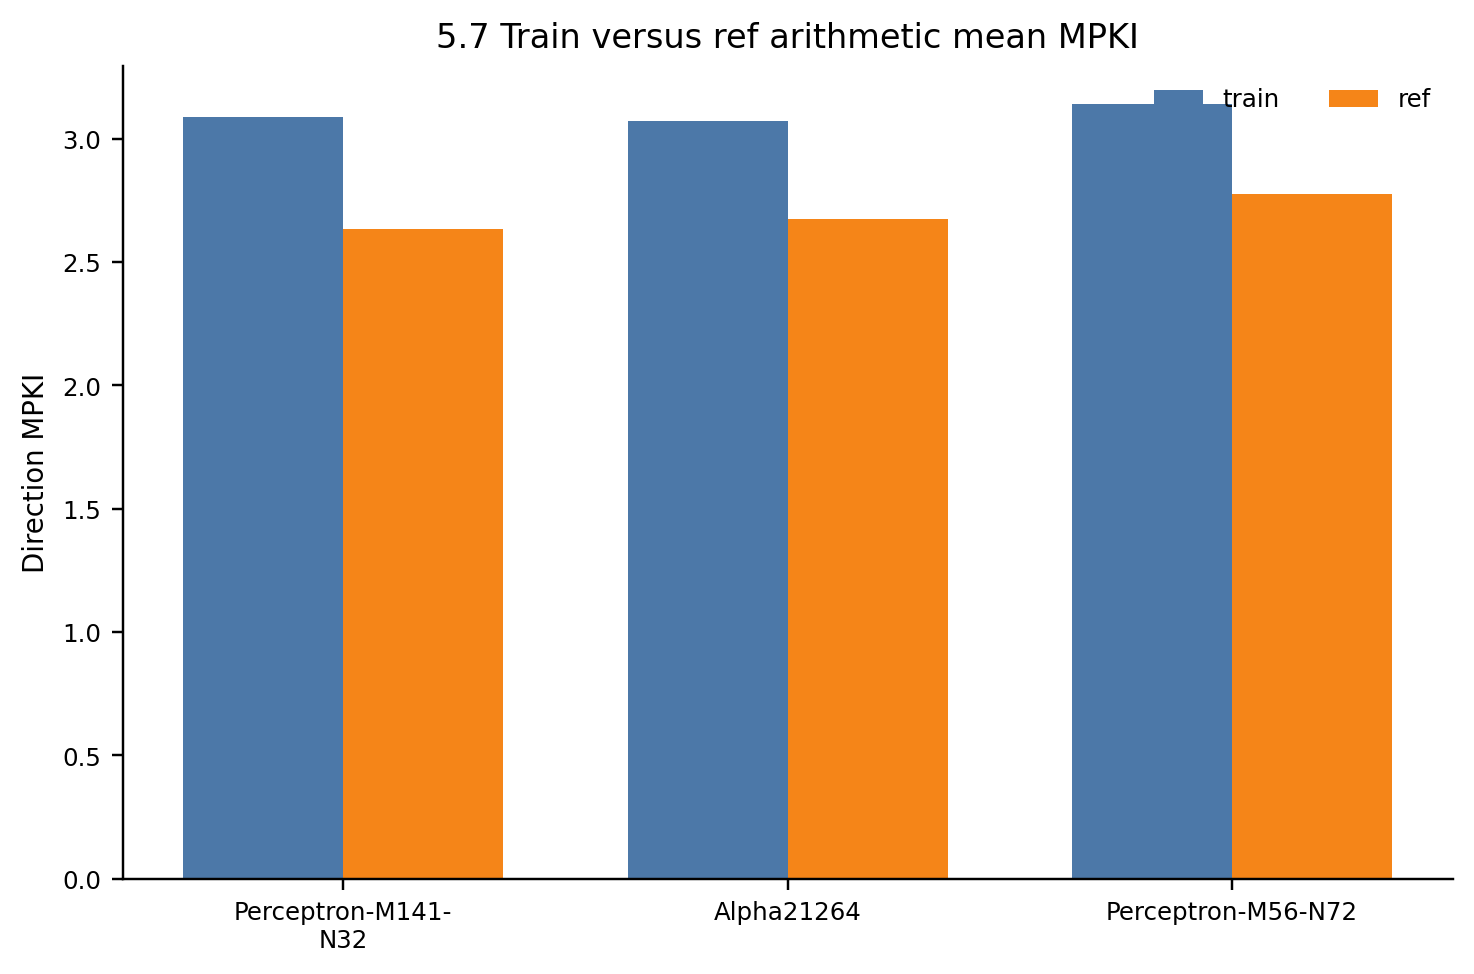
\includegraphics[width=0.72\linewidth]{5_7_train_vs_ref.png}
    \caption{Αριθμητικός μέσος του direction MPKI σε \texttt{train} και \texttt{ref} inputs για τους τρεις επιλεγμένους μηχανισμούς.}
    \label{fig:train_vs_ref}
\end{figure}

\begin{center}
\begin{tabular}{lrrrr}
\toprule
Predictor & Train mean & Ref mean & Train agg. & Ref agg. \\
\midrule
\texttt{Alpha21264} & 3.071 & 2.675 & 2.119 & 1.129 \\
\texttt{Perceptron-M141-N32} & 3.088 & 2.634 & 2.186 & 1.139 \\
\texttt{Perceptron-M56-N72} & 3.140 & 2.778 & 1.788 & 1.110 \\
\bottomrule
\end{tabular}
\captionof{table}{Σύγκριση \texttt{train} και \texttt{ref} για τους τρεις επιλεγμένους μηχανισμούς.}
\label{tab:train_ref}
\end{center}

\subsection{Σύγκριση συμπερασμάτων}

Στα \texttt{ref} inputs, και οι τρεις μηχανισμοί βελτιώνουν τον αριθμητικό μέσο του MPKI σε σχέση με τα \texttt{train} inputs. Η σειρά όμως αλλάζει οριακά. Ο \texttt{Perceptron-M141-N32} γίνεται πρώτος με 2.634 MPKI, ο \texttt{Alpha21264} ακολουθεί με 2.675 MPKI και ο \texttt{Perceptron-M56-N72} έχει 2.778 MPKI. Η διαφορά ανάμεσα στους δύο πρώτους είναι περίπου 0.04 MPKI, δηλαδή πολύ μικρή. Συνεπώς, δεν πρόκειται για ουσιαστική ανατροπή του συμπεράσματος, αλλά για μικρή μεταβολή μέσα στην κορυφαία ομάδα.

Η μικρή αυτή αλλαγή δείχνει ότι τα \texttt{train} inputs ήταν αρκετά αντιπροσωπευτικά για την αναγνώριση των καλύτερων predictors, αλλά όχι απαραίτητα για την ακριβή κατάταξη μεταξύ predictors με πολύ κοντινή επίδοση. Αυτό είναι αναμενόμενο, επειδή διαφορετικά input sets μπορούν να αλλάξουν τη σχετική συχνότητα συγκεκριμένων branch patterns.

\begin{figure}[htbp]
    \centering
    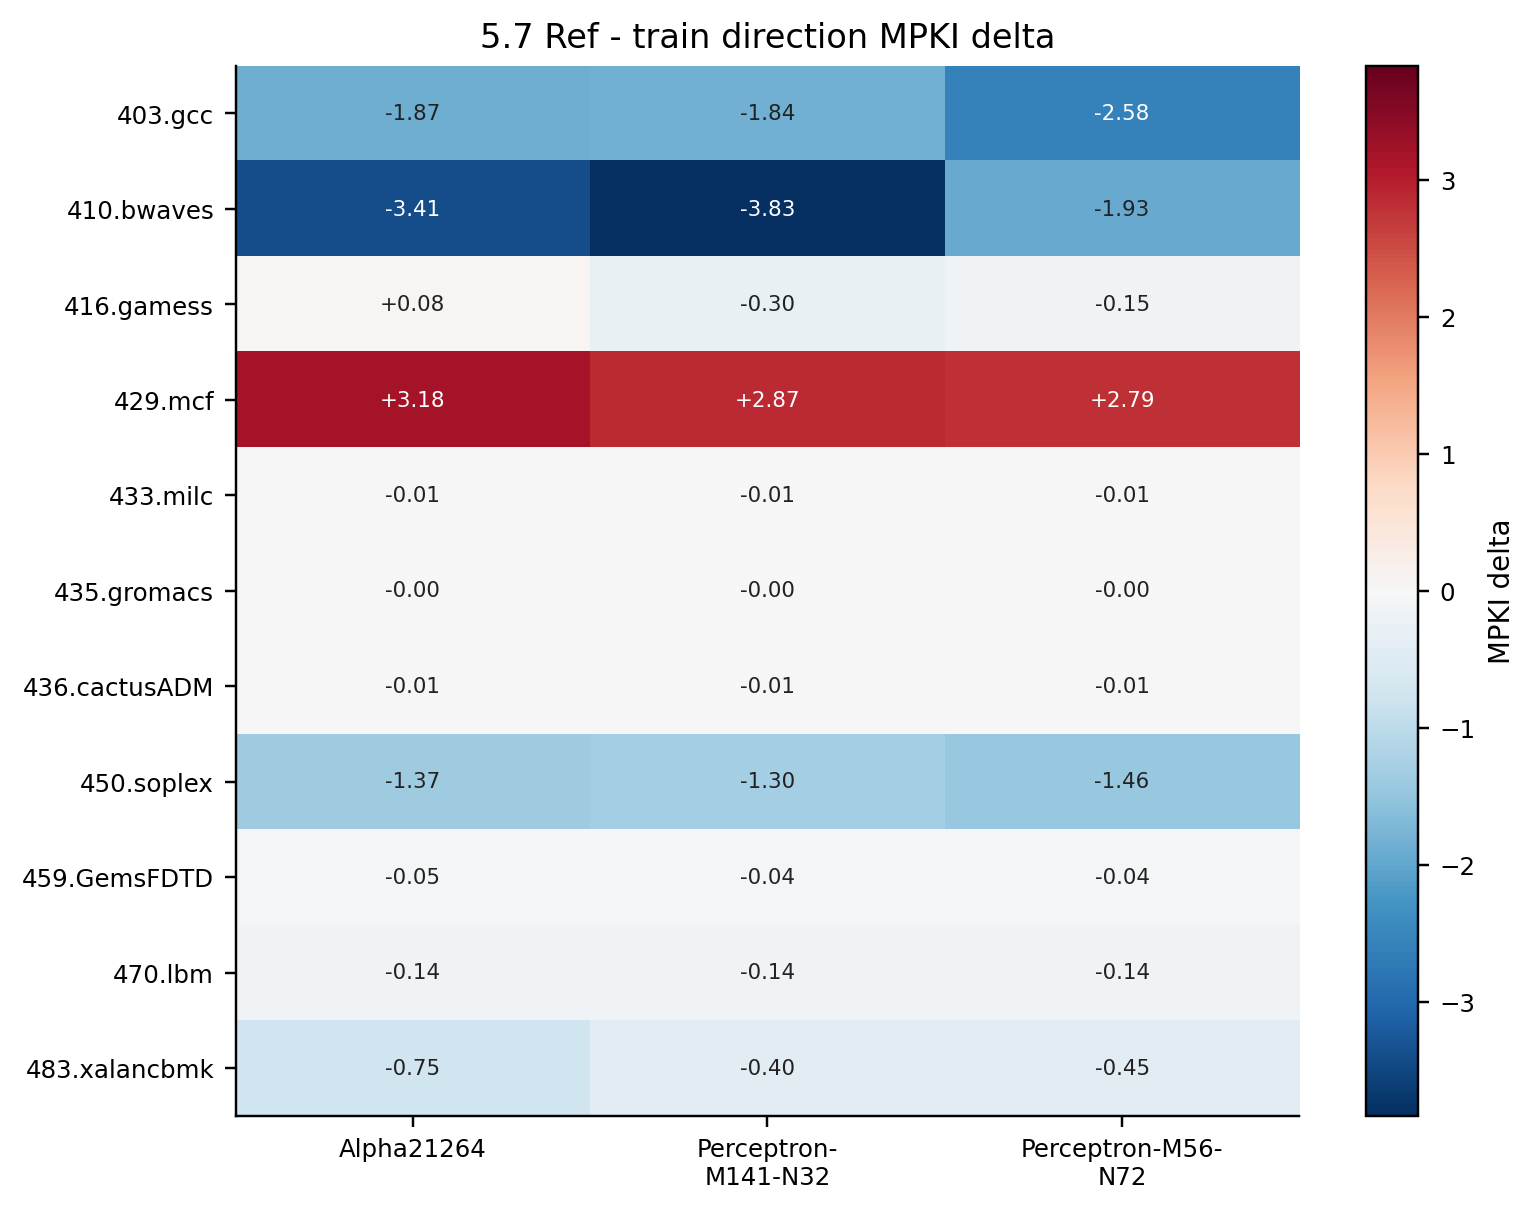
\includegraphics[width=0.76\linewidth]{5_7_ref_delta_heatmap.png}
    \caption{Μεταβολή του direction MPKI ανά benchmark από \texttt{train} σε \texttt{ref}. Αρνητική τιμή σημαίνει καλύτερη επίδοση στο \texttt{ref} input.}
    \label{fig:ref_delta}
\end{figure}

Το Σχήμα~\ref{fig:ref_delta} δείχνει αναλυτικά τη μεταβολή ανά benchmark. Η μεγαλύτερη επιδείνωση εμφανίζεται στο \texttt{429.mcf}, όπου και οι τρεις μηχανισμοί έχουν υψηλότερο MPKI στο \texttt{ref}. Αντίθετα, στα \texttt{403.gcc}, \texttt{410.bwaves} και \texttt{450.soplex}, η επίδοση βελτιώνεται. Υπάρχουν επίσης benchmarks όπως τα \texttt{433.milc}, \texttt{435.gromacs} και \texttt{436.cactusADM}, όπου οι μεταβολές είναι πρακτικά αμελητέες.

Σε aggregate MPKI η σειρά στα \texttt{ref} inputs είναι διαφορετική:
\[
    \texttt{Perceptron-M56-N72}, \quad
    \texttt{Alpha21264}, \quad
    \texttt{Perceptron-M141-N32},
\]
με τιμές 1.110, 1.129 και 1.139 αντίστοιχα. Αυτό επιβεβαιώνει ότι ο perceptron με μεγάλο global history length είναι πολύ ισχυρός στα benchmarks που έχουν μεγάλο βάρος σε δυναμικές εντολές. Ωστόσο, ο \texttt{Alpha21264} παραμένει η πιο ισορροπημένη τελική επιλογή. Ήταν πρώτος στο \texttt{train} mean, είναι πρακτικά ισοδύναμος με τον πρώτο στο \texttt{ref} mean, έχει καλύτερο \texttt{ref} aggregate από τον \texttt{Perceptron-M141-N32}, απαιτεί χαμηλότερο κόστος και έχει μικρότερη υπολογιστική πολυπλοκότητα ανά πρόβλεψη.

Άρα, το βασικό συμπέρασμα του 5.6.2 επιβεβαιώνεται. Η κορυφαία ομάδα predictors παραμένει η ίδια και στα \texttt{ref} inputs. Οι μικρές αλλαγές στη σειρά δείχνουν ότι η τελική επιλογή δεν πρέπει να βασίζεται μόνο σε μια αριθμητική τιμή, αλλά να λαμβάνει υπόψη και το hardware κόστος, την πολυπλοκότητα και τη σταθερότητα της επίδοσης.

\FloatBarrier
\section{Συνολικά συμπεράσματα}

Η άσκηση ανέδειξε ότι η πρόβλεψη διακλαδώσεων είναι σύνθετο πρόβλημα και δεν μπορεί να αξιολογηθεί με μία μόνο οπτική. Το 5.2 έδειξε ότι τα benchmarks έχουν διαφορετικό branch frequency και διαφορετικό μίγμα conditional branches, calls, returns και unconditional branches. Επομένως, η μικροαρχιτεκτονική πρέπει να αντιμετωπίζει ξεχωριστά την πρόβλεψη κατεύθυνσης, την πρόβλεψη target και την πρόβλεψη επιστροφών.

Στους απλούς n-bit predictors, ο 2-bit saturating counter παραμένει η καλύτερη πρακτική επιλογή όταν το hardware budget είναι σταθερό στα 32K bits. Ο 1-bit predictor έχει πολλά entries αλλά δεν έχει υστέρηση, ενώ ο 4-bit predictor έχει περισσότερη υστέρηση, αλλά λιγότερα entries και αυξημένο aliasing. Τα εναλλακτικά FSMs του Nair επιβεβαιώνουν ότι υπάρχουν μηχανές 4 καταστάσεων με σχεδόν ίδια επίδοση, αλλά δεν προσφέρουν ουσιαστικό πλεονέκτημα έναντι της απλής και καθιερωμένης μορφής του 2-bit predictor.

Στο BTB, η καλύτερη οργάνωση με βάση τον αριθμητικό μέσο του total miss MPKI είναι η \texttt{BTB-512-1}. Η παρατήρηση αυτή δείχνει ότι στα συγκεκριμένα traces η αύξηση του πλήθους entries είναι πιο σημαντική από την αύξηση του associativity. Στη RAS, η επιλογή 32 entries αποτελεί καλό αρχιτεκτονικό συμβιβασμό, επειδή προσφέρει σχεδόν όλο το όφελος των μεγαλύτερων stacks με αισθητά μικρότερο μέγεθος.

Οι perceptron predictors έδειξαν ότι το μεγάλο global history length μπορεί να μειώσει σημαντικά το MPKI. Στο 5.6.1, χωρίς αυστηρό περιορισμό κόστους, η διαμόρφωση \texttt{Perceptron-M1024-N72} πέτυχε πολύ χαμηλό mean MPKI, 2.287. Όμως, όταν το hardware budget περιορίζεται περίπου στα 32K bits, η σύγκριση γίνεται πιο ισορροπημένη και πρέπει να συνυπολογιστούν τόσο η ακρίβεια όσο και η πολυπλοκότητα υλοποίησης.

Στη συνολική σύγκριση του 5.6.2, ο \texttt{Alpha21264} ήταν η καλύτερη επιλογή με βάση τον αριθμητικό μέσο, με mean MPKI 3.071 και κόστος 29696 bits. Η επίδοσή του οφείλεται στον συνδυασμό local και global history και στη χρήση choice predictor, ο οποίος επιλέγει δυναμικά ποια συνιστώσα είναι πιο αξιόπιστη. Οι perceptron predictors ήταν πολύ κοντά, ειδικά οι \texttt{Perceptron-M141-N32} και \texttt{Perceptron-M56-N72}, όμως απαιτούν dot product σε κάθε πρόβλεψη και έχουν ελαφρώς μεγαλύτερο κόστος.

Το 5.7 έδειξε ότι τα συμπεράσματα από τα \texttt{train} inputs παραμένουν ουσιαστικά σταθερά και στα \texttt{ref} inputs. Η κορυφαία ομάδα predictors δεν αλλάζει. Ο \texttt{Perceptron-M141-N32} εμφανίζει οριακά καλύτερο \texttt{ref} mean MPKI, ενώ ο \texttt{Perceptron-M56-N72} έχει το καλύτερο \texttt{ref} aggregate MPKI. Παρ' όλα αυτά, ο \texttt{Alpha21264} παραμένει η πιο ισορροπημένη τελική επιλογή, επειδή συνδυάζει πολύ υψηλή ακρίβεια, χαμηλότερο κόστος, μικρότερη υπολογιστική πολυπλοκότητα και σταθερή συμπεριφορά στα δύο input sets.

Συνολικά, αν έπρεπε να επιλεγεί ένας μηχανισμός πρόβλεψης για υλοποίηση στο σύστημα, η τελική επιλογή θα ήταν ο \texttt{Alpha21264}. Προσφέρει τον καλύτερο συμβιβασμό ανάμεσα σε ακρίβεια, κόστος και πρακτικότητα, ενώ τα αποτελέσματα στα \texttt{ref} inputs επιβεβαιώνουν ότι η επιλογή αυτή δεν είναι απλώς αποτέλεσμα υπερπροσαρμογής στα \texttt{train} inputs.

\end{document}
